\documentclass[conference]{IEEEtran}

\usepackage[utf8]{inputenc}
\usepackage[T1]{fontenc}
\usepackage[spanish,es-nodecimaldot]{babel}
\usepackage{amsmath,amssymb}
\usepackage{graphicx}
\usepackage{booktabs}
\usepackage{siunitx}
\usepackage{microtype}
\usepackage{xcolor}
\usepackage{url}
\usepackage{balance}
\usepackage{eso-pic}

\sisetup{output-decimal-marker={,},per-mode=symbol}
\graphicspath{{figuras/}}

\title{Laboratorio 8: Sistemas de seguimiento con control integral en el espacio de estados}

\author{\IEEEauthorblockN{Aldo Pastore}
\IEEEauthorblockA{Carrera de Ingeniería Electrónica\\
Facultad de Ciencias y Tecnologías\\
Universidad Católica ``Nuestra Señora de la Asunción''\\
Asunción, Paraguay}}

\begin{document}
\maketitle

\begin{abstract}
Se diseñó un sistema digital de seguimiento para una planta analógica de segundo orden mediante realimentación de estados, acción integral y un estimador de estado actual. La síntesis se realizó con el modelo identificado y el modelo obtenido a partir de los componentes se utilizó para estudiar la sensibilidad ante diferencias de planta. Los escalones abiertos de validación se simularon sin reajustar parámetros: el modelo identificado redujo el RMSE conjunto de \SI{6.772}{mV} a \SI{5.756}{mV} y elevó el ajuste NRMSE medio de \SI{69.07}{\percent} a \SI{73.48}{\percent}. Se adoptó un período de muestreo de \SI{2}{ms} y se compararon controladores con polos integrales $0.60$ y $0.30$. MATLAB y Simulink permitieron comprobar los límites, la cuantización asimétrica del DAC y el anti-windup antes de implementar el algoritmo en un PSoC 5LP. Se verificó primero el modo \texttt{MONITOR}, luego se aplicaron escalones abiertos de $\pm\SI{50}{mV}$ y finalmente se ensayaron ambos lazos con una referencia de \SI{50}{mV}. El diseño lento alcanzó \SI{49}{mV} en régimen, con un error RMS de \SI{3.209}{mV}, subida de \SI{16}{ms} y sobrepasamiento de \SI{20}{\percent}; el rápido alcanzó \SI{48}{mV}, \SI{2.843}{mV} RMS, \SI{12}{ms} y \SI{18}{\percent}. No se activaron saturaciones, bloqueos de anti-windup ni fallas. El período se mantuvo entre \SI{1999}{\micro s} y \SI{2001}{\micro s}, mientras que el osciloscopio registró incrementos de \SI{47.2}{mV} y retornos próximos a cero. Al finalizar, el PSoC quedó programado en \texttt{MONITOR}.
\end{abstract}

\begin{IEEEkeywords}
acción integral, control digital, espacio de estados, estimador actual, PSoC 5LP, Simulink, seguimiento.
\end{IEEEkeywords}

\section{Introducción}
La realimentación de estados permite modificar la dinámica de una planta mediante la ubicación de polos, pero un precompensador calculado para el modelo nominal no elimina necesariamente el error permanente cuando existen perturbaciones, variaciones paramétricas o incertidumbre de modelado. Para obtener seguimiento robusto de referencias constantes se incorpora un estado integral del error. El sistema ampliado pasa de segundo a tercer orden y la señal de control combina el estado estimado de la planta con el estado integral.

\section{Objetivos y alcance}
Los objetivos son: seleccionar y justificar el período de muestreo; discretizar la planta mediante retención de orden cero; incorporar la integral del error; diseñar dos controladores variando la dinámica integral; implementar un estimador actual; comparar respuesta, esfuerzo y sensibilidad al modelo; y preparar una implementación segura en PSoC 5LP.

El alcance comprende el cálculo, las simulaciones MATLAB/Simulink, el firmware compilable, la prevalidación física segura, la revalidación bipolar en lazo abierto y el cierre de lazo con ambos diseños integrales. La placa se verificó inicialmente en modo \texttt{MONITOR}; luego se autorizaron corridas separadas de \SI{50}{mV} y \SI{-50}{mV} en lazo abierto y, finalmente, un pulso cerrado de \SI{50}{mV} para cada controlador, siempre con la planta energizada y tierra común. Finalizadas las capturas, el PSoC fue recompilado y programado nuevamente en \texttt{MONITOR}.

\section{Modelo y discretización}
\subsection{Modelo continuo nominal}
Con $x=[x_1\;x_2]^T$, $y=Cx$ y los valores $R_5=\SI{150}{k\ohm}$, $R_6=\SI{47}{k\ohm}$, $R_1=\SI{15}{k\ohm}$, $R_2=\SI{47}{k\ohm}$, $C_1=C_3=\SI{100}{nF}$, se empleó
\begin{equation}
\dot{x}=Fx+Gu,\qquad y=Cx,
\end{equation}
con
\begin{align}
F&=\begin{bmatrix}
-66.6667&0\\
-212.7660&-666.6667
\end{bmatrix},
&G&=\begin{bmatrix}-212.7660\\0\end{bmatrix},\\
C&=\begin{bmatrix}0&1\end{bmatrix}.
\end{align}

La discretización ZOH con $T_s=\SI{2}{ms}$ produjo
\begin{align}
A&=\begin{bmatrix}
0.875173319&0\\
-0.216870986&0.263597138
\end{bmatrix},\\
B&=\begin{bmatrix}-0.398383024\\0.057929374\end{bmatrix}.
\end{align}
Se verificaron $\operatorname{rank}\mathcal{C}(A,B)=2$ y $\operatorname{rank}\mathcal{O}(A,C)=2$.

\subsection{Selección del período de muestreo}
La frecuencia de muestreo es $f_s=\SI{500}{Hz}$. Para los polos dominantes deseados $0.80\pm j0.25$, la transformación $s=\ln(z)/T_s$ produce una frecuencia natural equivalente cercana a \SI{175}{rad/s}; así, $\omega_s/\omega_n\approx17.9$. El modo continuo identificado más rápido queda próximo a Nyquist, por lo que no se aproxima mediante reglas asintóticas: se conserva exactamente mediante ZOH. La selección de \SI{2}{ms} también deja margen suficiente para ejecutar la ISR; esta condición se comprueba experimentalmente con el temporizador de diagnóstico.

\subsection{Modelo identificado adoptado para síntesis}
La dinámica identificada se representó con ganancia $K=1.002941$, $\tau_1=\SI{9.06915}{ms}$ y $\tau_2=\SI{0.774399}{ms}$. Para mantener estados asociados a tensiones internas se conservó la ganancia nominal de la primera etapa y se asignó la segunda de modo que el producto reproduzca $K$. La discretización resultó
\begin{align}
A_{id}&=\begin{bmatrix}0.802095310&0\\-0.249628290&0.075573620\end{bmatrix},\\
B_{id}&=\begin{bmatrix}-0.631610700\\0.130459080\end{bmatrix}.
\end{align}
Estas matrices se usan para calcular $K_x$, $K_i$ y $L$. El nominal se simula como planta alternativa para medir sensibilidad al modelo.

\subsection{Validación independiente del modelo adoptado}
Los escalones abiertos medidos no se utilizaron para volver a identificar la planta: un único pulso por polaridad no excita suficientemente todos los parámetros de un modelo de segundo orden. Se emplearon, en cambio, como conjunto de validación independiente. Para cada adquisición se restó la mediana de las 32 muestras de pretrigger y se simularon, sin ajuste adicional, el modelo nominal y el identificado con el mando cuantizado realmente aplicado. La ventana de evaluación comprende el frente, la meseta y el retorno inicial.

\begin{table*}[!t]
\caption{Validación abierta independiente de los modelos}
\label{tab:validacion-modelos}
\centering
\small
\begin{tabular}{llrrrr}
\toprule
Ensayo & Modelo & RMSE [mV] & Ajuste NRMSE [\%] & Meseta predicha [mV] & Sesgo de meseta [mV]\\
\midrule
Positivo & Nominal & 6.214 & 69.41 & 46.85 & -1.15\\
Positivo & Identificado & 5.777 & 71.56 & 46.14 & -1.86\\
Negativo & Nominal & 7.289 & 68.74 & -53.98 & -3.98\\
Negativo & Identificado & 5.735 & 75.40 & -53.16 & -3.16\\
Ambos & Nominal & 6.772 & 69.07 & -- & --\\
Ambos & Identificado & 5.756 & 73.48 & -- & --\\
\bottomrule
\end{tabular}
\end{table*}

\begin{figure*}[!t]
\centering
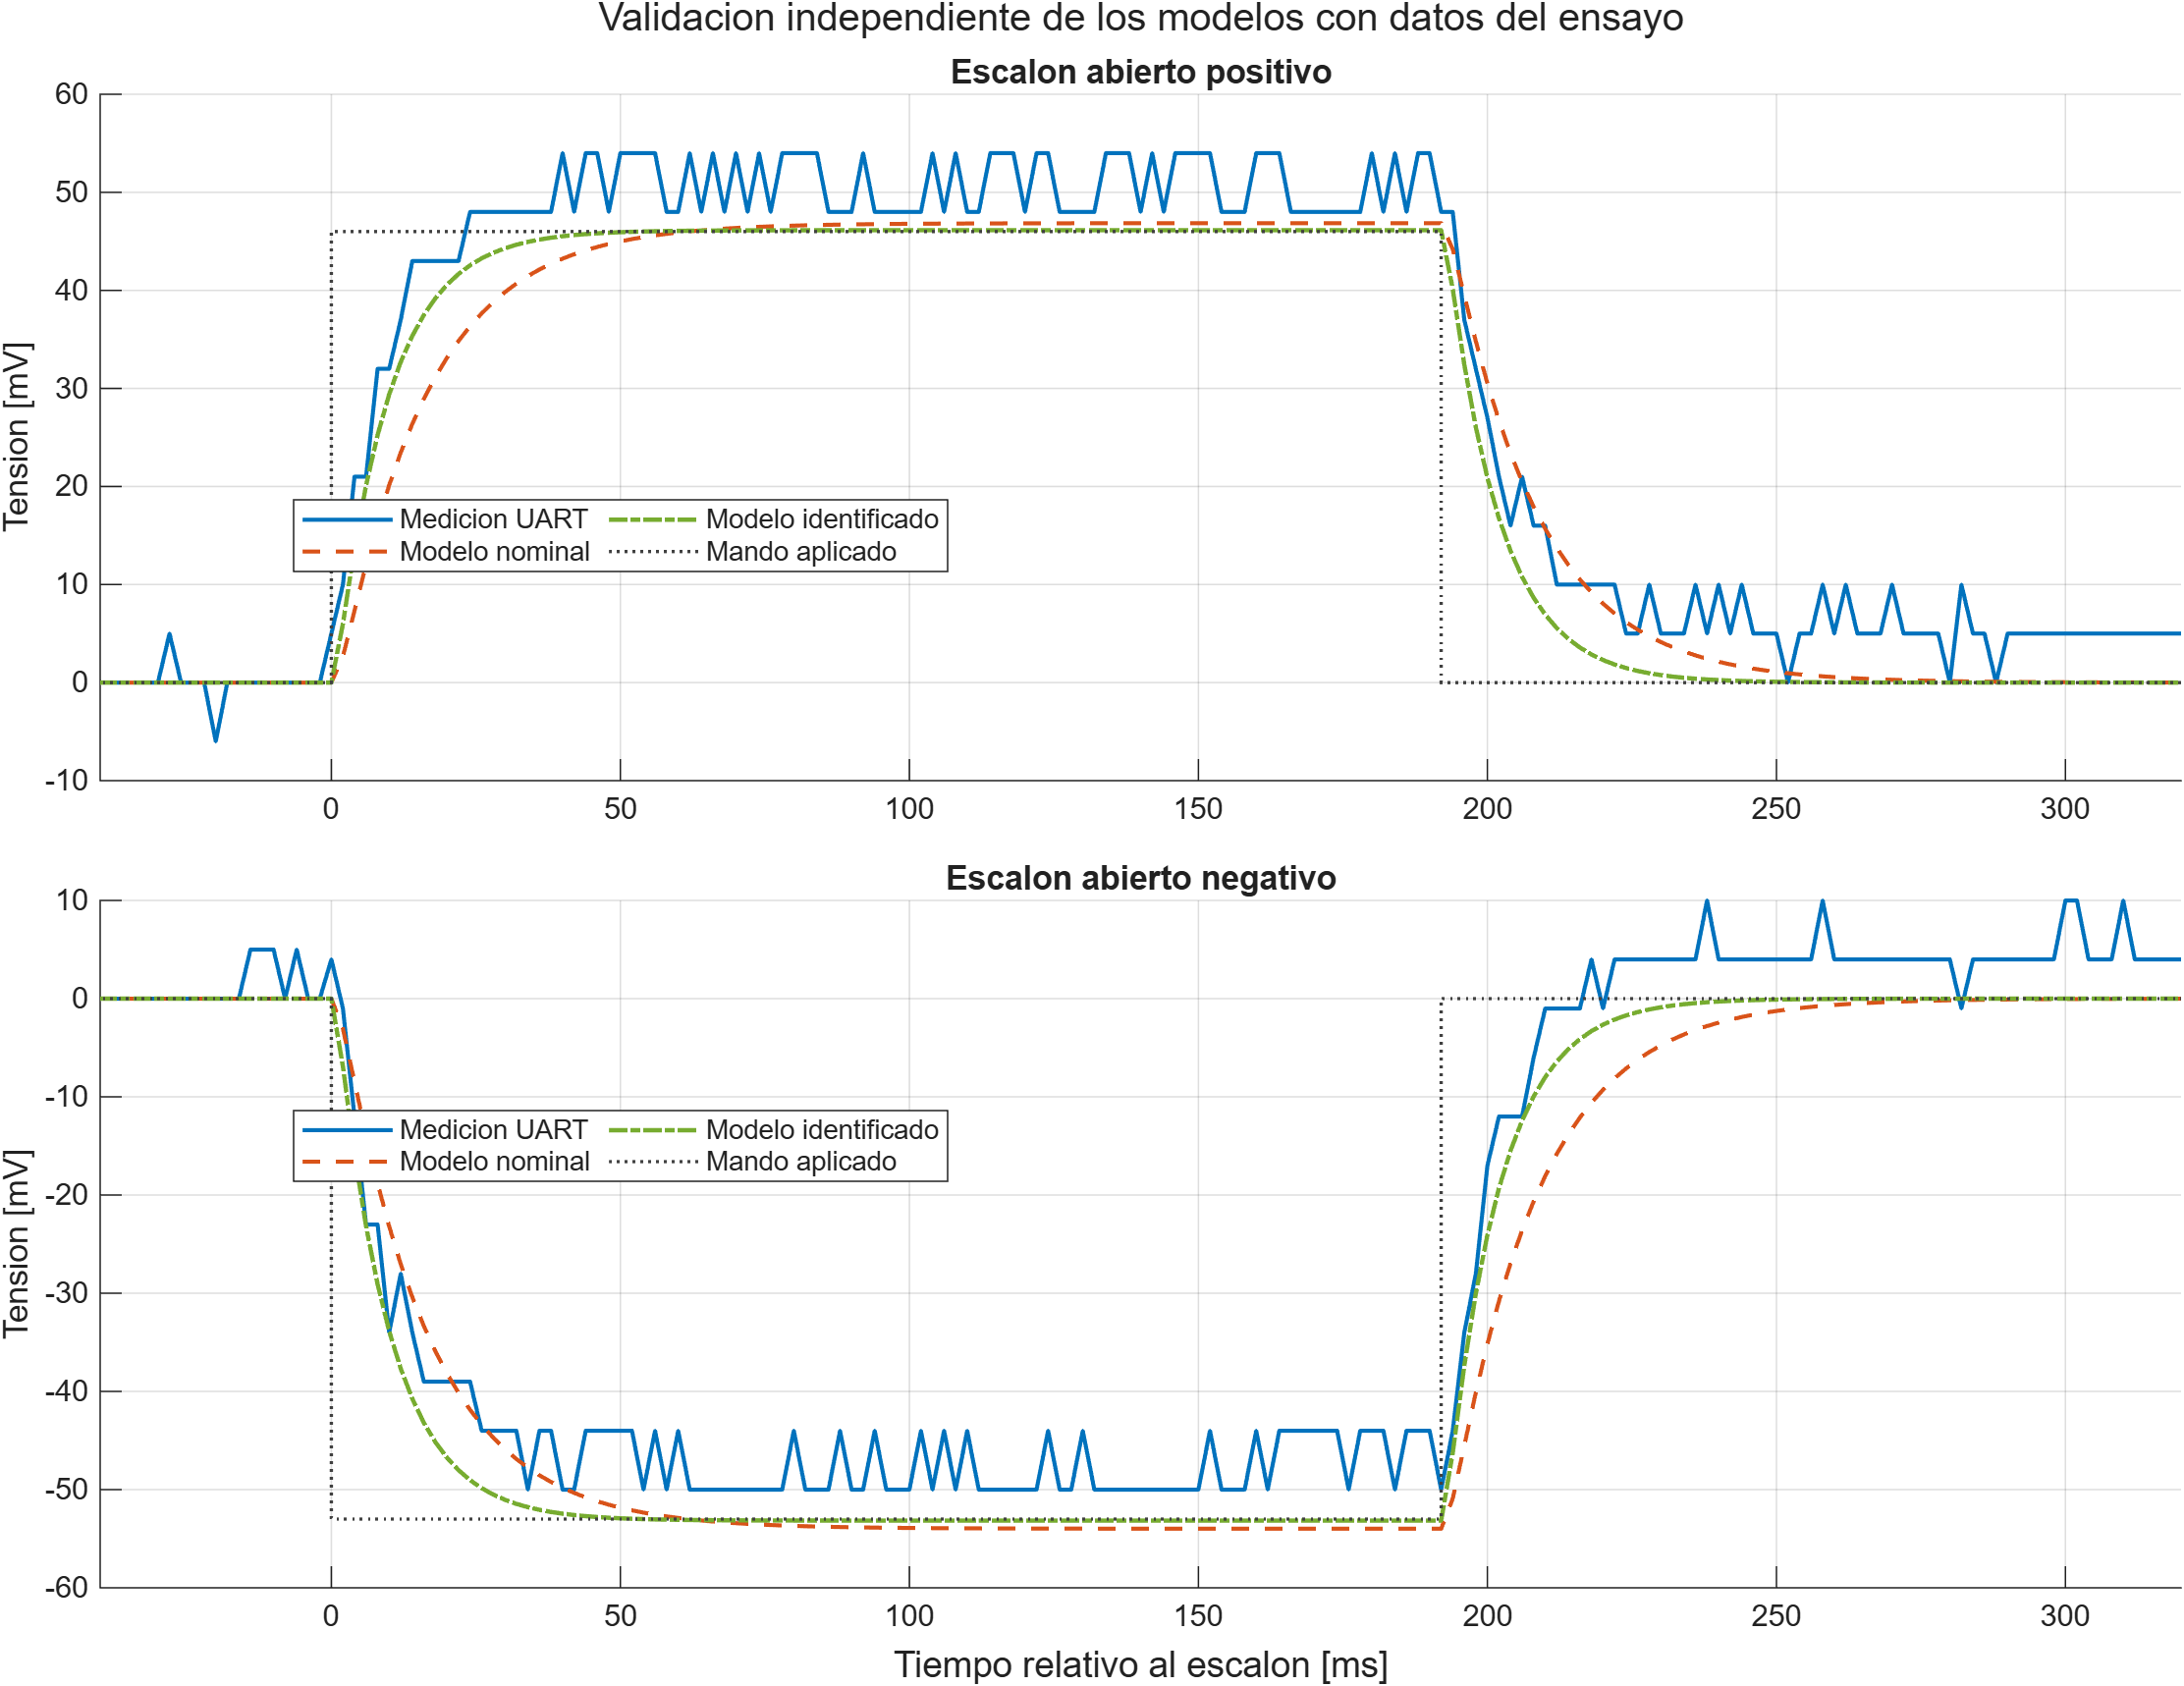
\includegraphics[width=0.94\textwidth]{validacion_modelos_abierto_lab8.png}
\caption{Validación abierta de los modelos. Se comparan las respuestas calculadas con la salida UART, utilizando el mando efectivamente aplicado y sin reajustar parámetros.}
\label{fig:validacion-modelos}
\end{figure*}

El modelo identificado presenta menor RMSE en ambas polaridades y un ajuste medio \SI{4.41}{puntos porcentuales} superior. En el escalón positivo el nominal aproxima levemente mejor la meseta, pero reproduce peor el frente; en el negativo el identificado mejora simultáneamente la dinámica y el sesgo. Estos pulsos no constituyen una nueva identificación, pero sí confirman que el modelo identificado representa mejor la dinámica observada y resulta adecuado para la síntesis.

\section{Control integral y estimador}
El estado integral se define por
\begin{equation}
\xi[k+1]=\xi[k]+r[k]-y[k].
\end{equation}
El sistema aumentado para diseño es
\begin{equation}
A_a=\begin{bmatrix}A&0\\-C&1\end{bmatrix},\qquad
B_a=\begin{bmatrix}B\\0\end{bmatrix},
\end{equation}
y se verificó $\operatorname{rank}\mathcal{C}(A_a,B_a)=3$. La ley implementada es
\begin{equation}
u[k]=-K_x\hat{x}[k]-K_i\xi[k].
\end{equation}

Los polos dominantes se fijaron en $0.80\pm j0.25$. Al conservar este par, la comparación aísla el efecto del tercer polo: $0.60$ produce una corrección integral más gradual y $0.30$, más próxima al origen, una dinámica integral más rápida. La Tabla~\ref{tab:ganancias} muestra las ganancias obtenidas.

\begin{table}[!t]
\caption{Ganancias de los controladores integrales}
\label{tab:ganancias}
\centering
\small
\begin{tabular}{lccc}
\toprule
Diseño & $z_i$ & $K_x$ & $K_i$\\
\midrule
Lento & 0.60 & $[1.654554\;5.539690]$ & $-0.223450$\\
Rápido & 0.30 & $[0.591027\;2.690254]$ & $-0.391037$\\
\bottomrule
\end{tabular}
\end{table}

Se utilizó un estimador actual con polos $0.20\pm j0.10$ y
\begin{equation}
L=\begin{bmatrix}-1.860494424&0.175152235\end{bmatrix}^{T}.
\end{equation}
En cada muestra se calcula la innovación, se corrige el estado antes del control y se predice el siguiente estado con el mando aplicado:
\begin{align}
\tilde y[k]&=y[k]-C\hat{x}^{-}[k],\\
\hat{x}[k]&=\hat{x}^{-}[k]+L\tilde y[k],\\
\hat{x}^{-}[k+1]&=A\hat{x}[k]+Bu_{\mathrm{ap}}[k].
\end{align}

La Fig.~\ref{fig:polos} verifica explícitamente la ubicación. Los polos calculados coinciden con los objetivos con error máximo $9.1\times10^{-16}$ para ambos controladores y $2.5\times10^{-16}$ para el observador. El módulo del par dominante es $0.8382$ y el del observador $0.2236$; por tanto, la estimación converge con una dinámica considerablemente más rápida que la del lazo de control.

\begin{figure*}[!t]
\centering
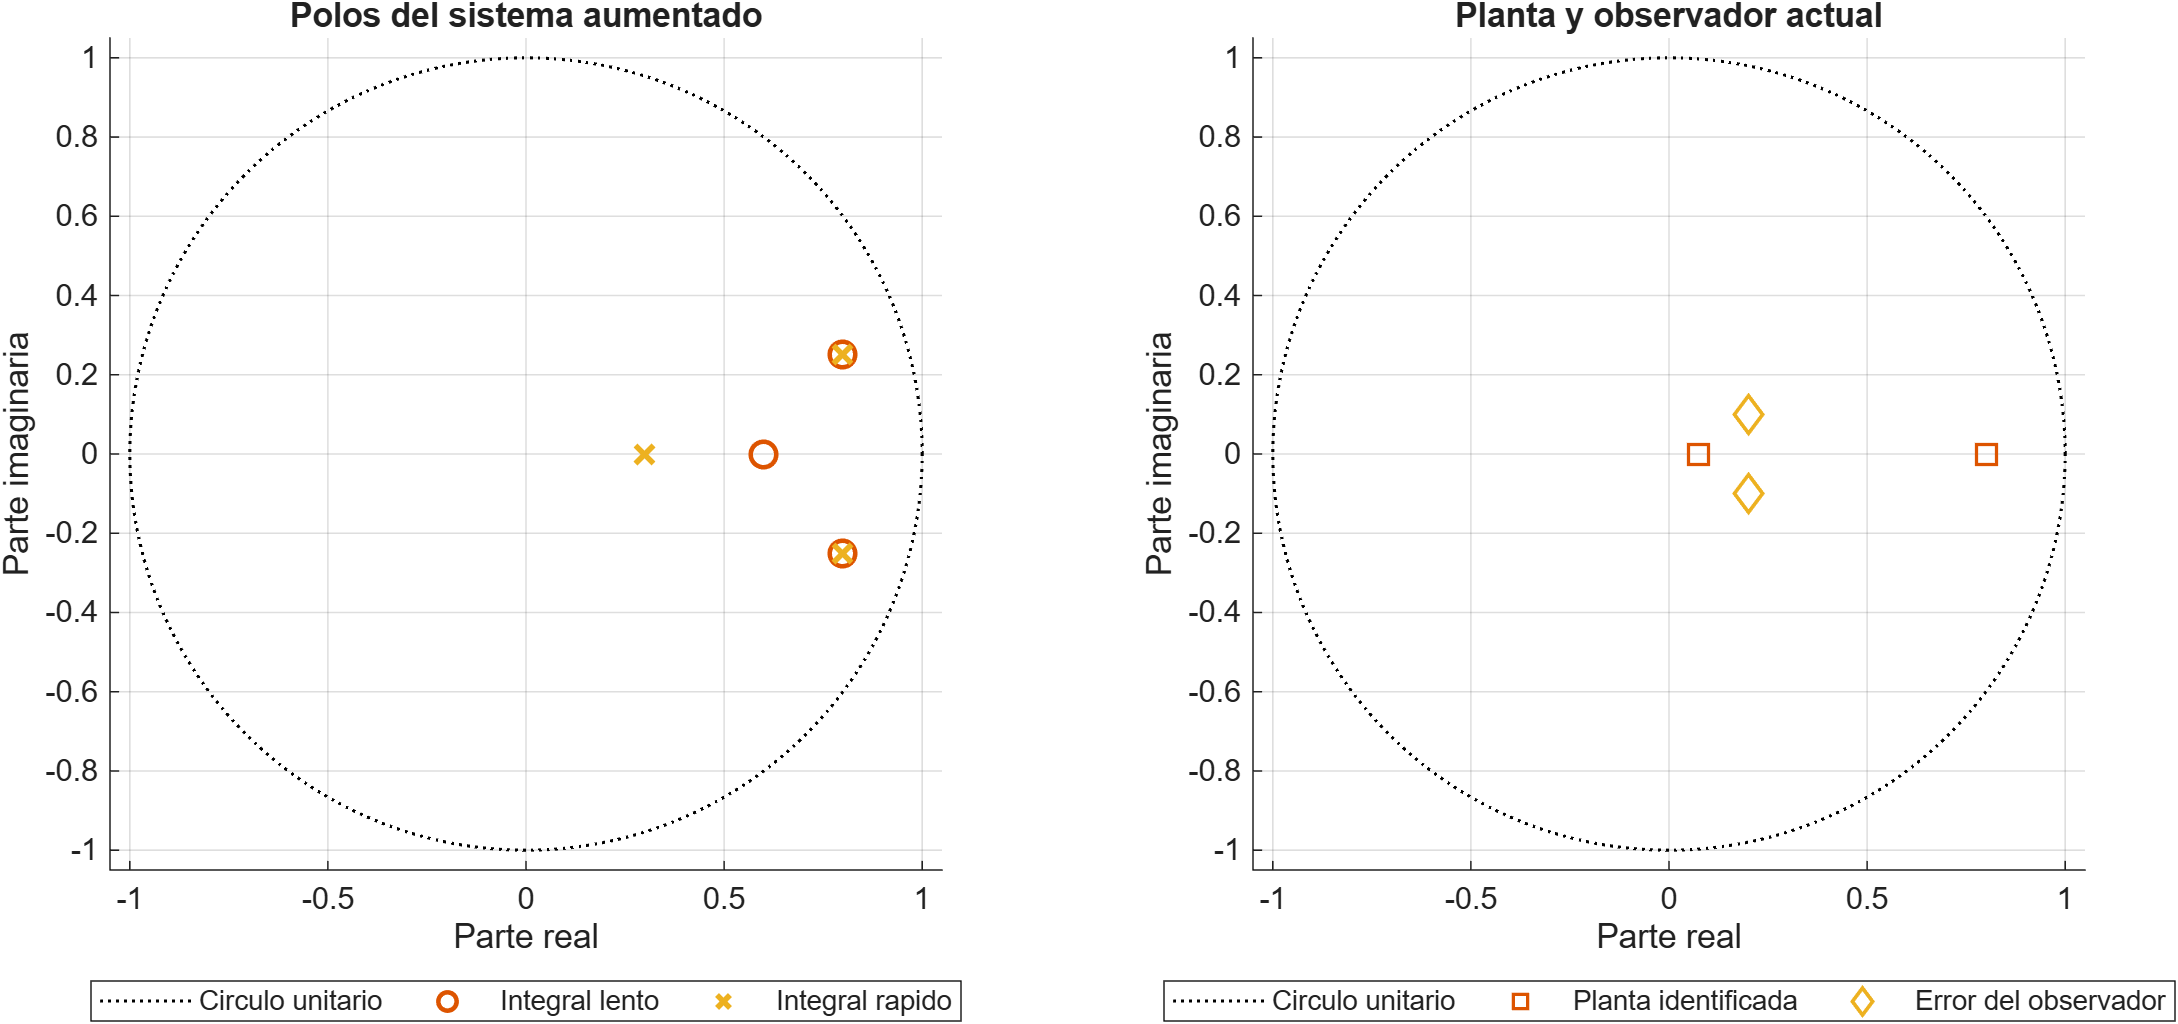
\includegraphics[width=0.93\textwidth]{mapa_polos_lab8.png}
\caption{Polos obtenidos en el plano $z$. Los dos controladores comparten el par dominante y difieren únicamente en el polo integral; el observador actual conserva sus polos dentro del círculo unitario.}
\label{fig:polos}
\end{figure*}

Los límites precuantización se fijaron en $u\in[-115,107]$~mV. El anti-windup congela la integral cuando el mando ideal está saturado y el error empuja en la misma dirección; permite, en cambio, la integración necesaria para salir de saturación.

\section{Implementación MATLAB y Simulink}
La referencia de prueba es un pulso de \SI{50}{mV}, activo desde \SI{64}{ms} hasta \SI{664}{ms}. MATLAB calcula controlador y observador con $A_{id},B_{id}$ y luego evalúa ambos diseños sobre las plantas identificada y nominal. Se incluyen los límites y el DAC asimétrico modelado: \SI{15.370448}{mV} por código en la rama positiva y \SI{10.560423}{mV} por código en la negativa.

El modelo Simulink implementa explícitamente la integral, el observador actual identificado, la ley de control, los límites mediante bloques mínimo/máximo, la lógica de anti-windup y la planta discreta. Un script de inicialización selecciona \texttt{lento}/\texttt{rapido} y \texttt{nominal}/\texttt{identificada}; el valor predeterminado de planta es \texttt{identificada}. Otro script ejecuta los cuatro casos con objetos \texttt{SimulationInput}. El modelo se comprobó sin puertos ni líneas desconectados.

\begin{figure*}[!t]
\centering
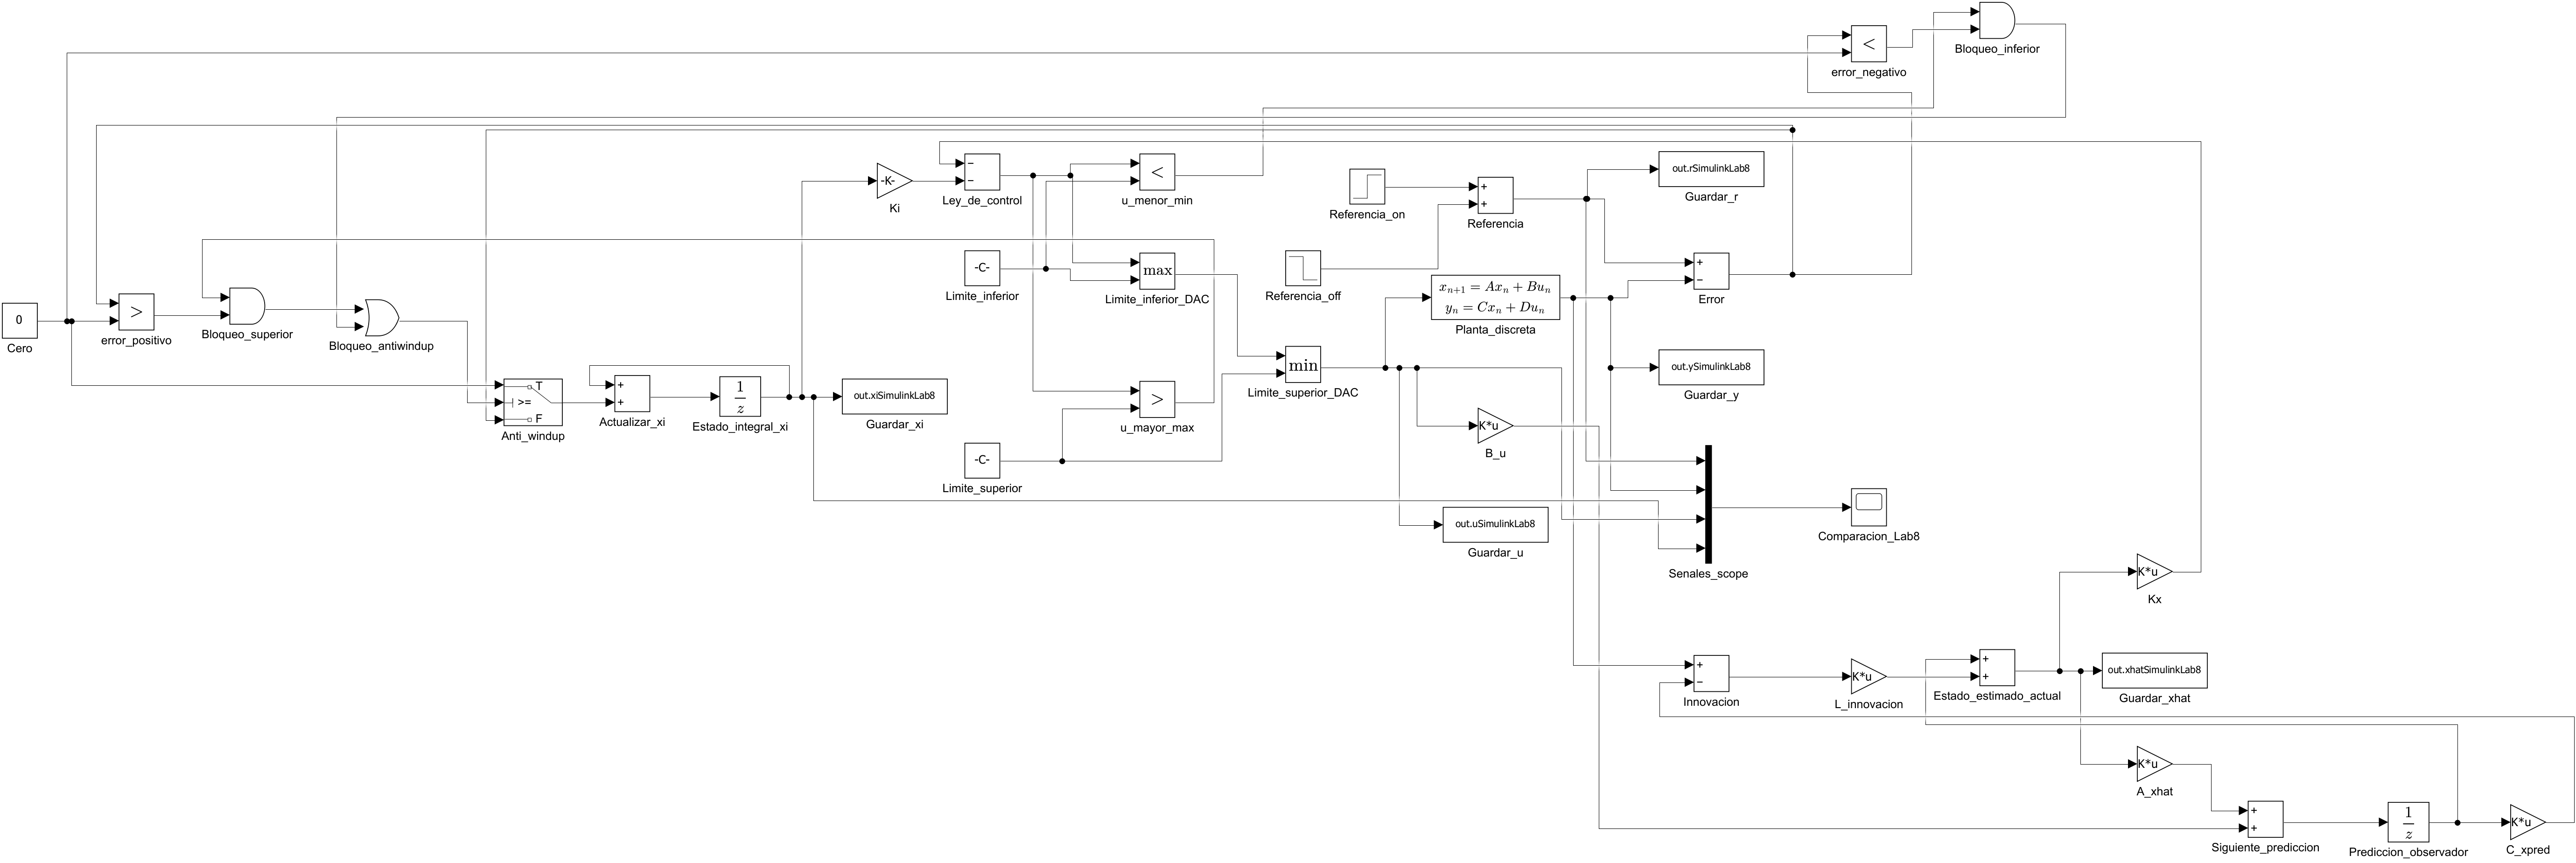
\includegraphics[width=0.98\textwidth]{diagrama_simulink_lab8.png}
\caption{Modelo Simulink: referencia, planta, estimador actual, control integral, saturación y anti-windup.}
\label{fig:simulink}
\end{figure*}

\section{Implementación PSoC 5LP}
La implementación se organizó en el workspace \texttt{Lab8.cywrk}. El \emph{TopDesign} contiene el ADC, los dos DAC, los temporizadores, la UART y los pines de diagnóstico. La capa de hardware concentra la conversión entre cuentas y voltios, mientras que el núcleo de control se mantiene en archivos independientes para poder probar sus operaciones numéricas fuera de la placa. Las matrices $A_{id}$ y $B_{id}$, las ganancias y los límites se declaran en un único punto del programa para evitar diferencias entre la simulación y el firmware.

La ISR de \SI{2}{ms} realiza: lectura ADC; corrección de cero con 32 muestras de pretrigger; estimación actual; cálculo del control; anti-windup; cuantización mediante la HAL; corrección de la predicción con la tensión efectivamente aplicada; registro de estados, integral, innovación, códigos DAC y tiempos. La referencia se retira en la muestra 333 y la adquisición finaliza en la muestra 600.

Se implementaron cuatro niveles de protección:
\begin{enumerate}
\item modo predeterminado \texttt{MONITOR}, con DAC en cero;
\item enclavamientos de compilación para escalón y lazo cerrado;
\item límites físicos, detección ADC, comprobación numérica y vigilancia de tiempo de ISR;
\item parada segura que detiene el temporizador y fuerza ambos DAC a cero.
\end{enumerate}

Se compilaron ambos caminos de control integral, la configuración abierta limitada y la configuración final segura. Los builds finalizaron sin errores. La imagen integral lenta ocupó 10120 de 262144 bytes de Flash (\SI{3.9}{\percent}) y la rápida 10128 bytes; ambas emplearon 33825 de 65536 bytes de SRAM (\SI{51.6}{\percent}). Al terminar, la imagen \texttt{MONITOR} ocupó 9392 bytes de Flash con la misma SRAM, incluyendo \SI{2048}{bytes} de pila y \SI{128}{bytes} de \emph{heap}. Esta imagen segura fue programada y verificada nuevamente en el PSoC 5LP.

\section{Resultados de simulación}
\subsection{DAC cuantizado}
La Tabla~\ref{tab:cuantizado} resume la simulación MATLAB con DAC cuantizado. ``--'' indica que la salida no entró y permaneció en la banda del \SI{2}{\percent} antes de terminar el pulso; no debe interpretarse como un tiempo infinito. No hubo saturaciones precuantización.

\begin{table*}[!t]
\caption{Respuesta simulada con DAC cuantizado}
\label{tab:cuantizado}
\centering
\scriptsize
\begin{tabular}{llrrrrrrr}
\toprule
Diseño & Planta & $\rho$ & $t_r$ [ms] & $t_s$ [ms] & $M_p$ [\%] & $e_{ss}$ [mV] & $u_{\min}$ [mV] & $u_{\max}$ [mV]\\
\midrule
Lento & Nominal & 0.9383 & 16 & -- & 29.90 & 0.450 & -31.681 & 76.852\\
Lento & Identificada & 0.8382 & 14 & -- & 15.66 & 0.365 & -21.121 & 61.482\\
Rápido & Nominal & 0.9268 & 12 & 598 & 30.82 & -0.138 & -42.242 & 92.223\\
Rápido & Identificada & 0.8382 & 10 & 596 & 15.03 & -0.055 & -21.121 & 76.852\\
\bottomrule
\end{tabular}
\end{table*}

\begin{figure*}[!t]
\centering
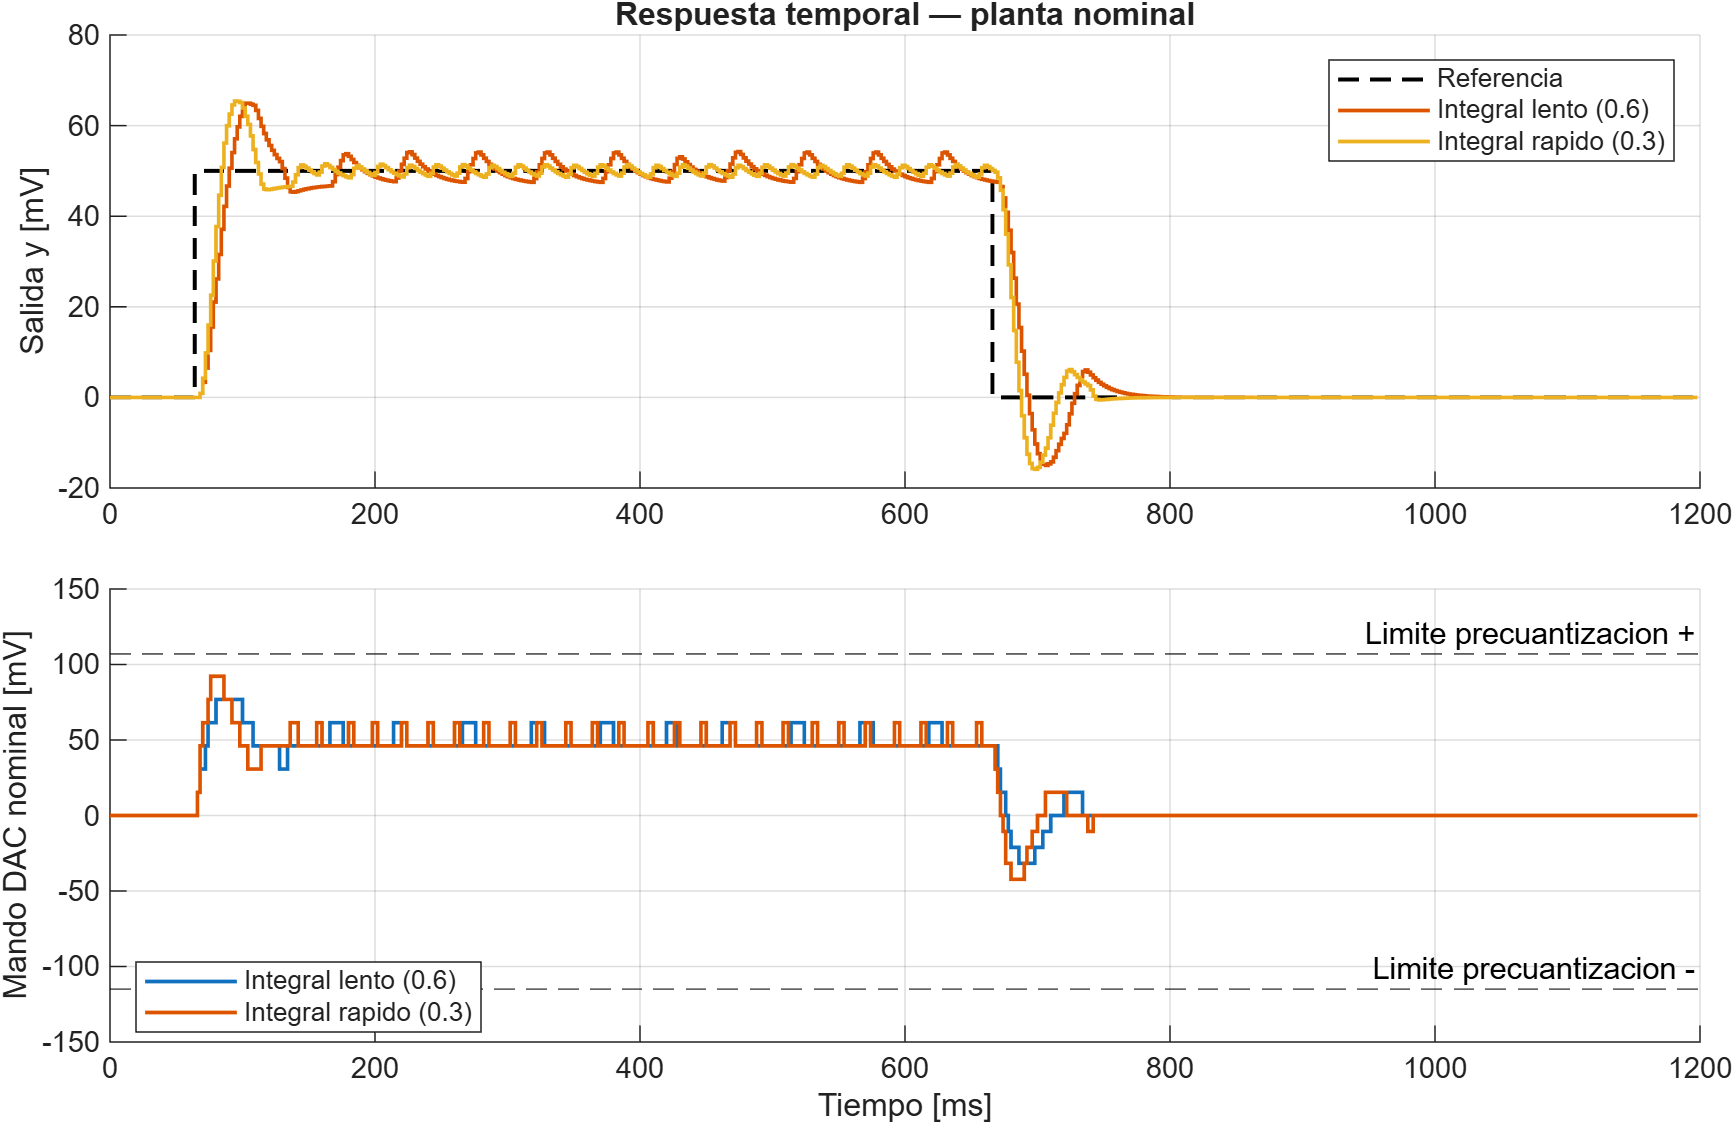
\includegraphics[width=0.92\textwidth]{comparacion_integral_nominal.png}
\caption{Comparación de los dos diseños sobre la planta nominal con el modelo cuantizado del DAC.}
\label{fig:nominal}
\end{figure*}

\begin{figure*}[!t]
\centering
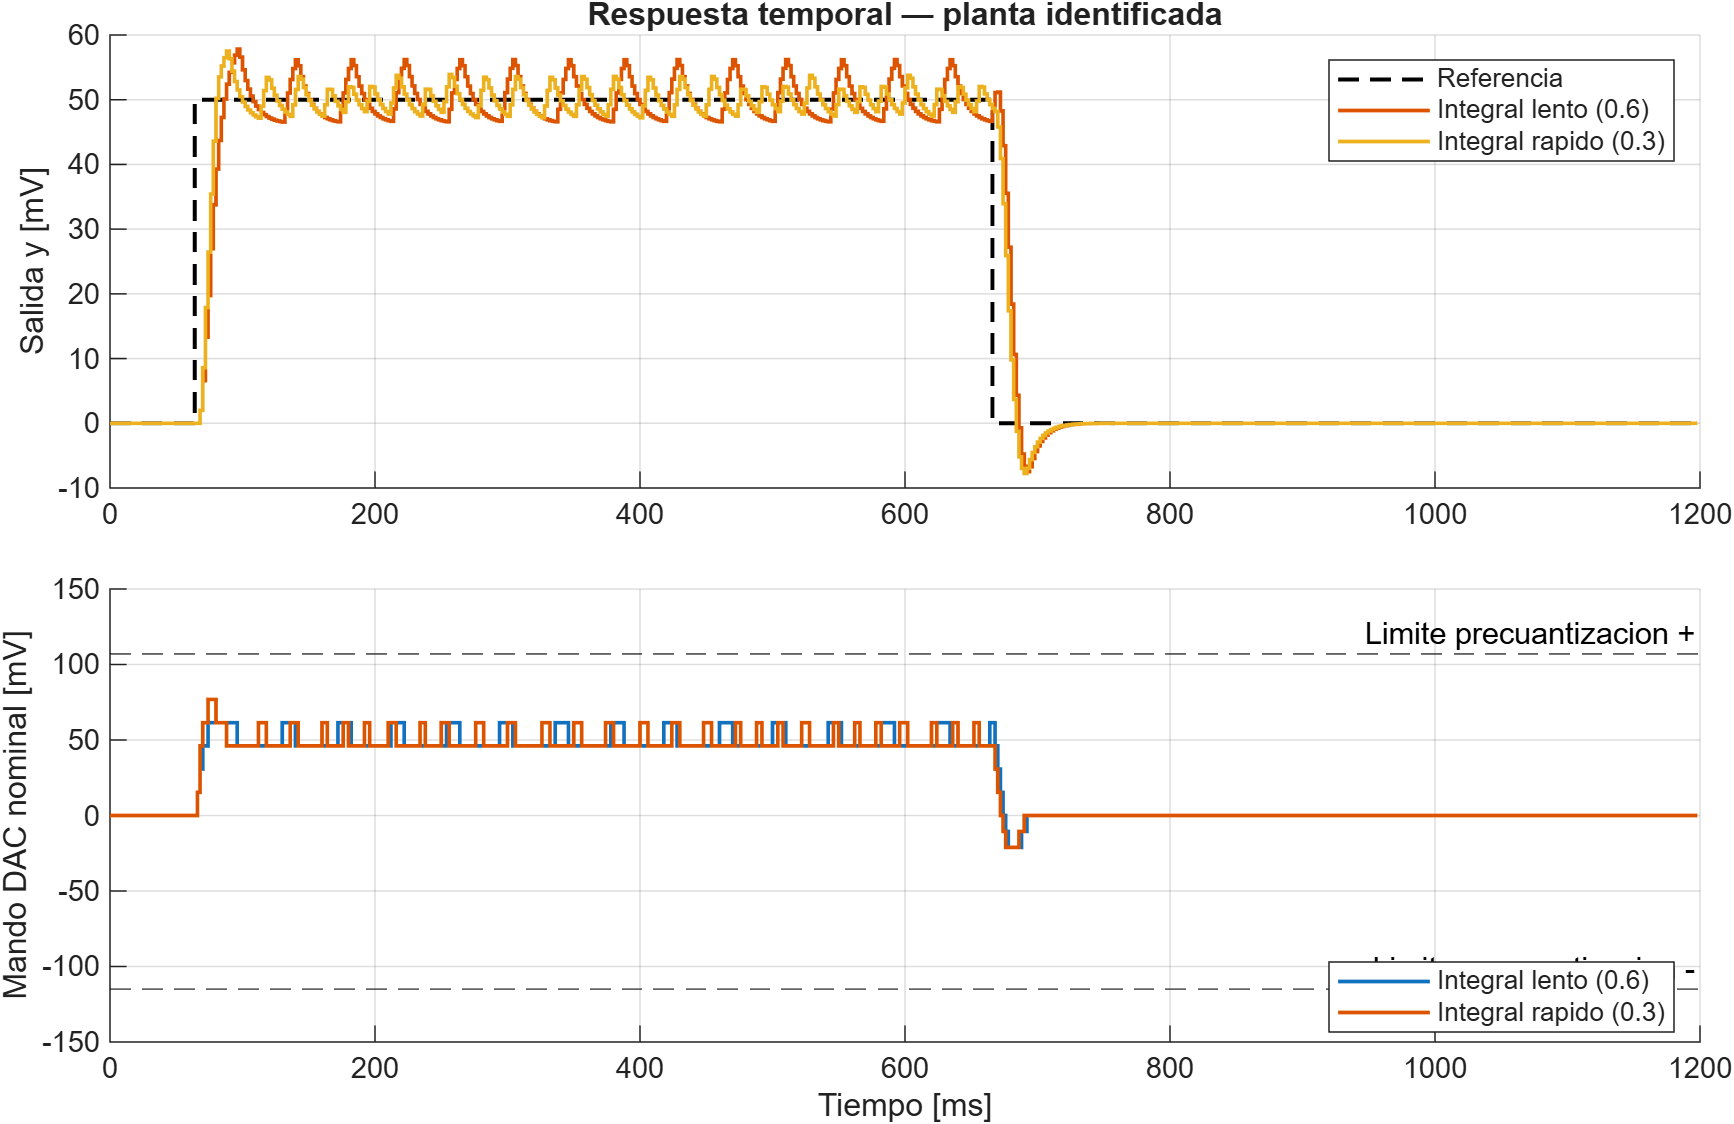
\includegraphics[width=0.92\textwidth]{comparacion_integral_identificada.png}
\caption{Comparación de los dos diseños sobre la planta identificada utilizada para la síntesis.}
\label{fig:identificada}
\end{figure*}

El error RMS en la ventana de régimen fue, respectivamente, 2.0880, 3.0793, 0.8575 y \SI{1.5417}{mV} para lento/nominal, lento/identificada, rápido/nominal y rápido/identificada. La cuantización produce un ciclo límite pequeño incluso cuando el sistema lineal ideal tiene error prácticamente nulo.

\subsection{Verificación independiente en Simulink}
La Tabla~\ref{tab:simulink} presenta los cuatro casos con DAC ideal limitado. Los máximos de mando coinciden con la simulación ideal de MATLAB dentro de la precisión numérica, lo que verifica la implementación por bloques.

\begin{table}[!t]
\caption{Resumen Simulink con DAC ideal limitado}
\label{tab:simulink}
\centering
\scriptsize
\begin{tabular}{llrrr}
\toprule
Diseño & Planta & $y_{\max}$ & $u_{\min}$ & $u_{\max}$\\
 & & [mV] & [mV] & [mV]\\
\midrule
Lento & Nominal & 65.287 & -32.473 & 81.561\\
Lento & Identificada & 55.895 & -19.672 & 69.525\\
Rápido & Nominal & 66.372 & -43.534 & 92.623\\
Rápido & Identificada & 57.634 & -24.734 & 74.588\\
\bottomrule
\end{tabular}
\end{table}

\section{Resultados experimentales}
\label{sec:experimental}
\subsection{Modo MONITOR}
La primera medición se realizó con CH1 del RIGOL conectado a J5 y CH2 a J7, sondas configuradas en 10X, tierra común y firmware \texttt{MONITOR}. MATLAB coordinó el puerto COM4 a 57600~bit/s con el RIGOL DS1202Z-E mediante VISA. Después del reinicio sincronizado se registraron 600 filas UART, 1200 puntos por canal y la captura de pantalla original del instrumento. Como el modo seguro no genera una transición, el disparo se forzó después de comprobar el estado \texttt{WAIT}; esto no modifica los datos descargados y queda registrado en los metadatos.

\begin{table}[!t]
\caption{Prevalidación física MONITOR}
\label{tab:monitor}
\centering
\small
\begin{tabular}{lrr}
\toprule
Magnitud & Resultado & Criterio\\
\midrule
Muestras UART & 600 & 600\\
Media de $y_{rel}$ [mV] & $-0.257$ & informativo\\
Desviación de $y_{rel}$ [mV] & 1.884 & informativo\\
Pico absoluto de $y_{rel}$ [mV] & 11.0 & informativo\\
Período mediano [\si{\micro s}] & 2000 & 2000\\
Intervalo mínimo/máximo [\si{\micro s}] & 1999/2001 & estable\\
Tiempo máximo de ISR [\si{\micro s}] & 52 & $<2000$\\
Flags no nulos & 0 & 0\\
Pico DAC $+/-$ [código] & 0/0 & 0/0\\
\bottomrule
\end{tabular}
\end{table}

La Fig.~\ref{fig:monitor-resumen} relaciona los datos UART con las formas de onda descargadas. La media/desviación observada por el RIGOL fue \SI{15.923}{mV}/\SI{3.576}{mV} en CH1 y \SI{11.383}{mV}/\SI{12.035}{mV} en CH2. Estas magnitudes corresponden al reposo de esta conexión y todavía no constituyen una caracterización dinámica.

\begin{figure*}[!t]
\centering
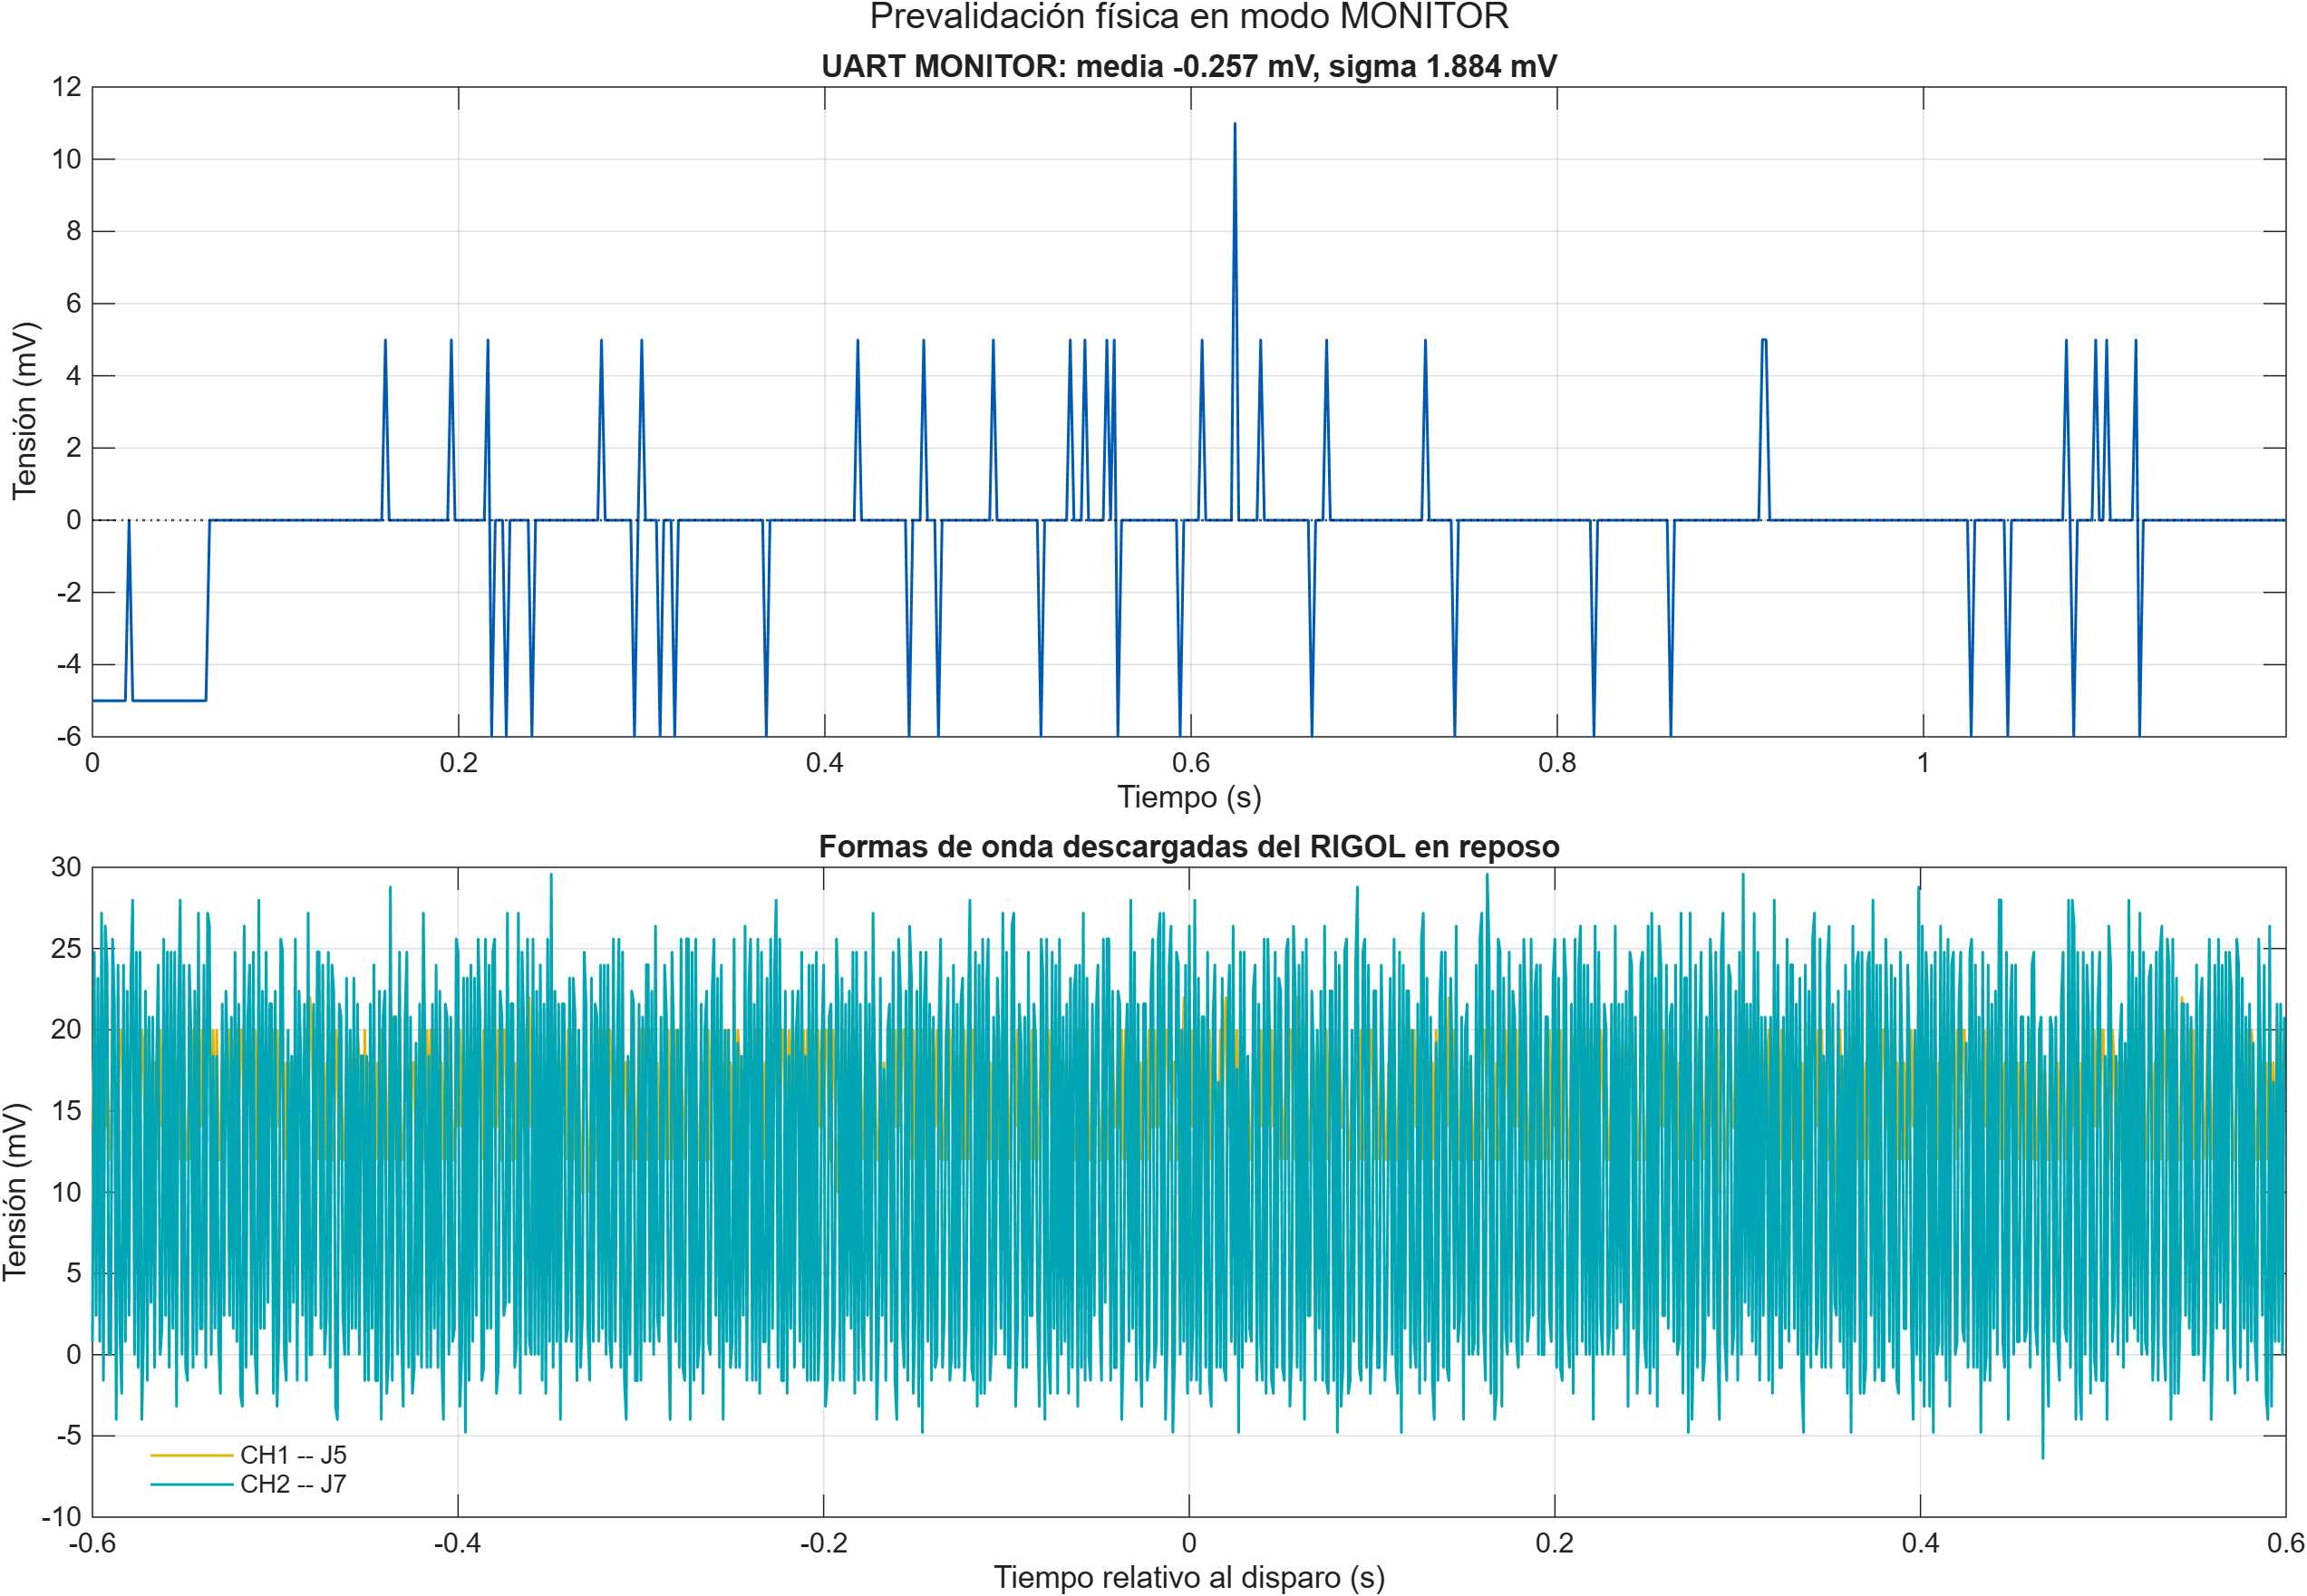
\includegraphics[width=0.88\textwidth]{monitor_fisico_lab8_resumen.png}
\caption{Prevalidación física: salida relativa registrada por UART y formas de onda CH1--J5/CH2--J7 descargadas del RIGOL.}
\label{fig:monitor-resumen}
\end{figure*}

\begin{figure*}[!t]
\centering
\includegraphics[width=0.84\textwidth]{pantalla_rigol_monitor_original.png}
\caption{Captura original del RIGOL DS1202Z-E durante la prevalidación MONITOR. Se conserva sin recreación ni posprocesado.}
\label{fig:rigol-original}
\end{figure*}

\subsection{Revalidación bipolar en lazo abierto}
Después de comprobar alimentación, tierra común y salida nula, se compiló el modo abierto y se ejecutaron por separado escalones de \SI{50}{mV} y \SI{-50}{mV}. Cada pulso se aplicó entre las muestras 32 y 127, es decir, durante 96 períodos o \SI{192}{ms}, y el firmware forzó luego ambos DAC a cero. Cada adquisición sincronizada reunió 600 filas UART, 1200 puntos por canal y la pantalla original del RIGOL. Entre ensayos se volvió a cargar la configuración \texttt{MONITOR}.

La Tabla~\ref{tab:abierto-bipolar} resume los resultados. La cuantización asimétrica seleccionó los códigos $+3$ y $-5$, equivalentes a \SI{46}{mV} y \SI{-53}{mV}. El RIGOL midió en J5 incrementos de \SI{47.6}{mV} y \SI{-54.0}{mV}. La cadena ADC/UART alcanzó \SI{43}{mV} y \SI{-49}{mV}, con ganancias de 0.935 y 0.925 y tiempos de subida de \SI{22}{ms} y \SI{24}{ms}. El canal J7 indicó \SI{36.8}{mV} y \SI{-42.4}{mV}, equivalentes a ganancias 0.773 y 0.785 respecto de J5. No se registraron banderas y el peor tiempo de ISR ocupó sólo \SI{2.95}{\percent} de $T_s$ en ambas polaridades.

\begin{table}[!t]
\caption{Ensayos abiertos de $\pm50$ mV}
\label{tab:abierto-bipolar}
\centering
\scriptsize
\begin{tabular}{lrr}
\toprule
Magnitud & $+50$ mV & $-50$ mV\\
\midrule
Escalón nominal [mV] & 46 & -53\\
$\Delta$J5 [mV] & 47.6 & -54.0\\
Salida UART tardía [mV] & 43.0 & -49.0\\
$\Delta$J7 RIGOL [mV] & 36.8 & -42.4\\
Ganancia UART & 0.935 & 0.925\\
Ganancia RIGOL & 0.773 & 0.785\\
Tiempo de subida UART [ms] & 22 & 24\\
Pulso [muestras/ms] & 96/192 & 96/192\\
Período mín./med./máx. [$\mu$s] & 1999/2000/2001 & 1999/2000/2001\\
Tiempo máximo de ISR [$\mu$s] & 59 & 59\\
Pico DAC $+/-$ [código] & 3/0 & 0/5\\
Flags no nulos & 0 & 0\\
\bottomrule
\end{tabular}
\end{table}

Los mismos datos permiten verificar la escala del DAC en los códigos utilizados durante el ensayo. La Tabla~\ref{tab:escala-dac} compara el incremento medido en J5 por código con el valor empleado en el modelo. La diferencia fue de \SI{3.23}{\percent} en la rama positiva y \SI{2.27}{\percent} en la negativa. Esta comprobación corresponde al punto de operación utilizado; no reemplaza una calibración multipunto de toda la escala.

\begin{table}[!t]
\caption{Comprobación de la escala del DAC en el punto de ensayo}
\label{tab:escala-dac}
\centering
\scriptsize
\begin{tabular}{lrrrr}
\toprule
Rama & Código & Modelo & Medición & Diferencia\\
 & & [mV/cód.] & [mV/cód.] & [\%]\\
\midrule
Positiva & 3 & 15.370 & 15.867 & 3.23\\
Negativa & 5 & 10.560 & 10.800 & 2.27\\
\bottomrule
\end{tabular}
\end{table}

\begin{figure*}[!t]
\centering
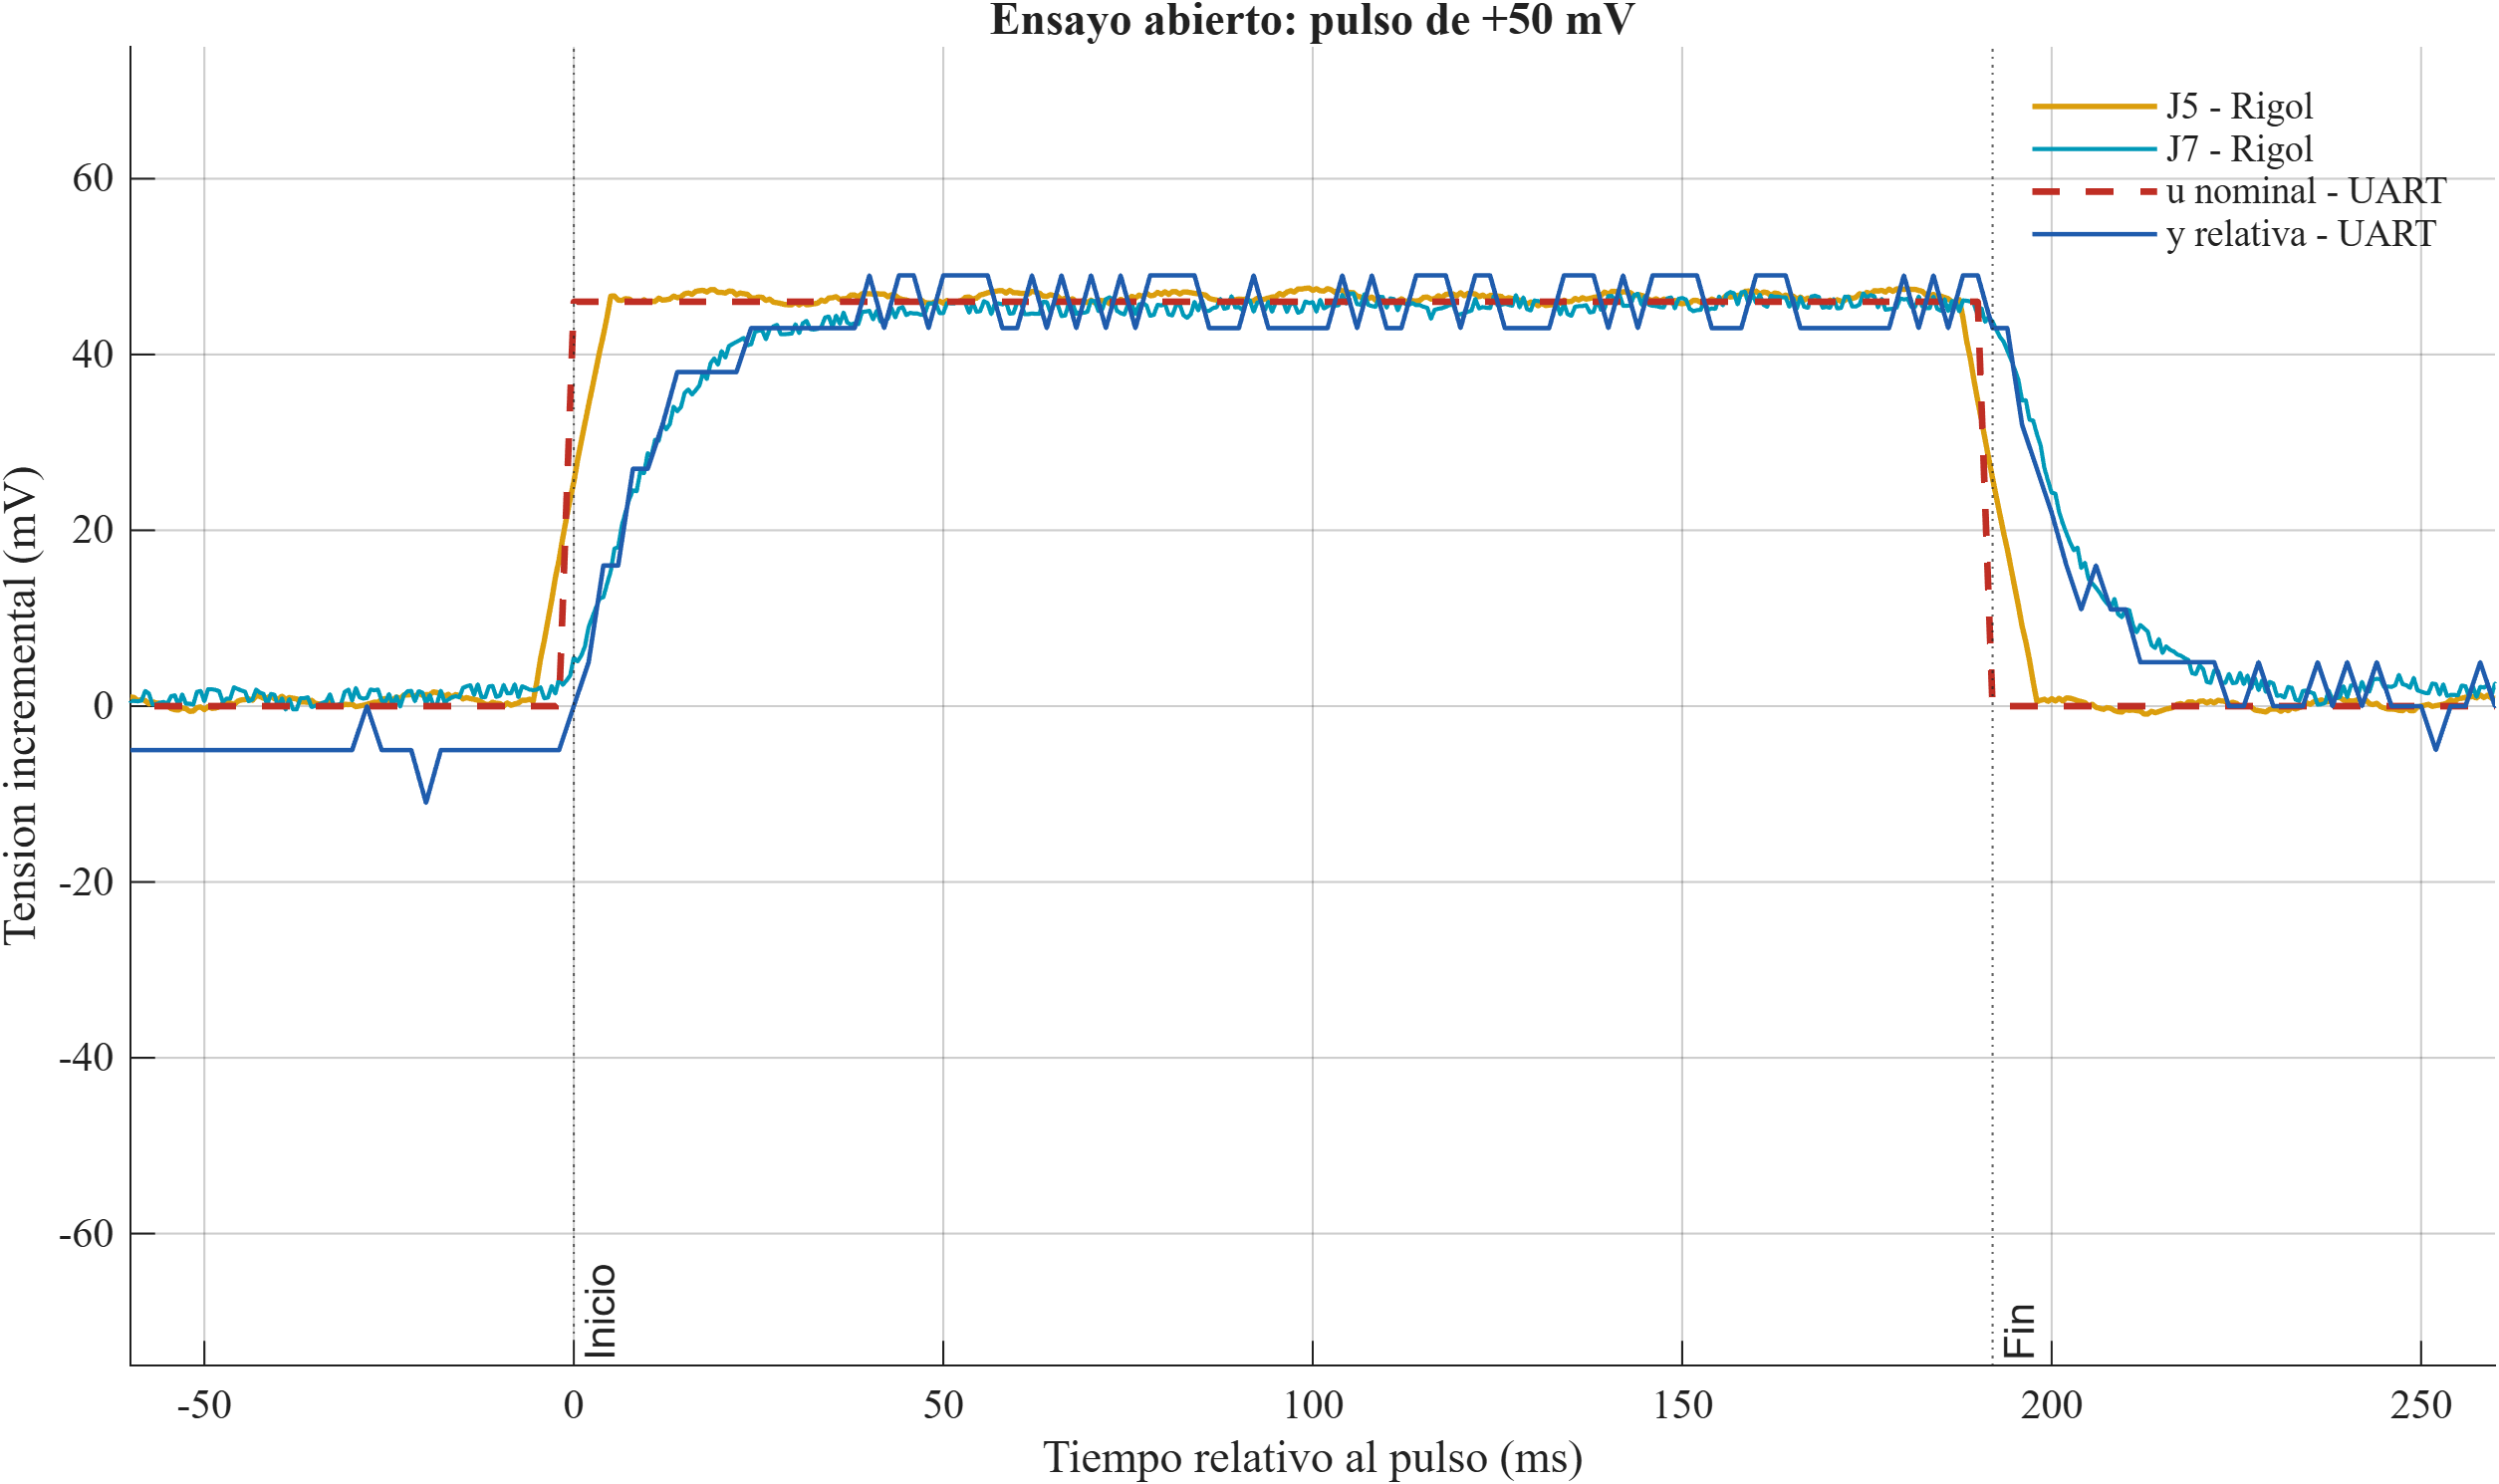
\includegraphics[width=0.94\textwidth]{ensayo_abierto_pos_50mV.png}
\caption{Ensayo abierto positivo: comparación temporal entre J5 y J7 descargados del RIGOL y las variables de entrada y salida registradas por UART.}
\label{fig:abierto-pos}
\end{figure*}

\begin{figure*}[!t]
\centering
\includegraphics[width=0.84\textwidth]{pantalla_rigol_abierto_pos_50mV_original.png}
\caption{Pantalla original del RIGOL durante el ensayo abierto de +50 mV. Se observan ambos flancos y la meseta completa. El disparo forzado desplazó el origen temporal al flanco descendente, sin recortar el pulso.}
\label{fig:rigol-abierto-pos}
\end{figure*}

\begin{figure*}[!t]
\centering
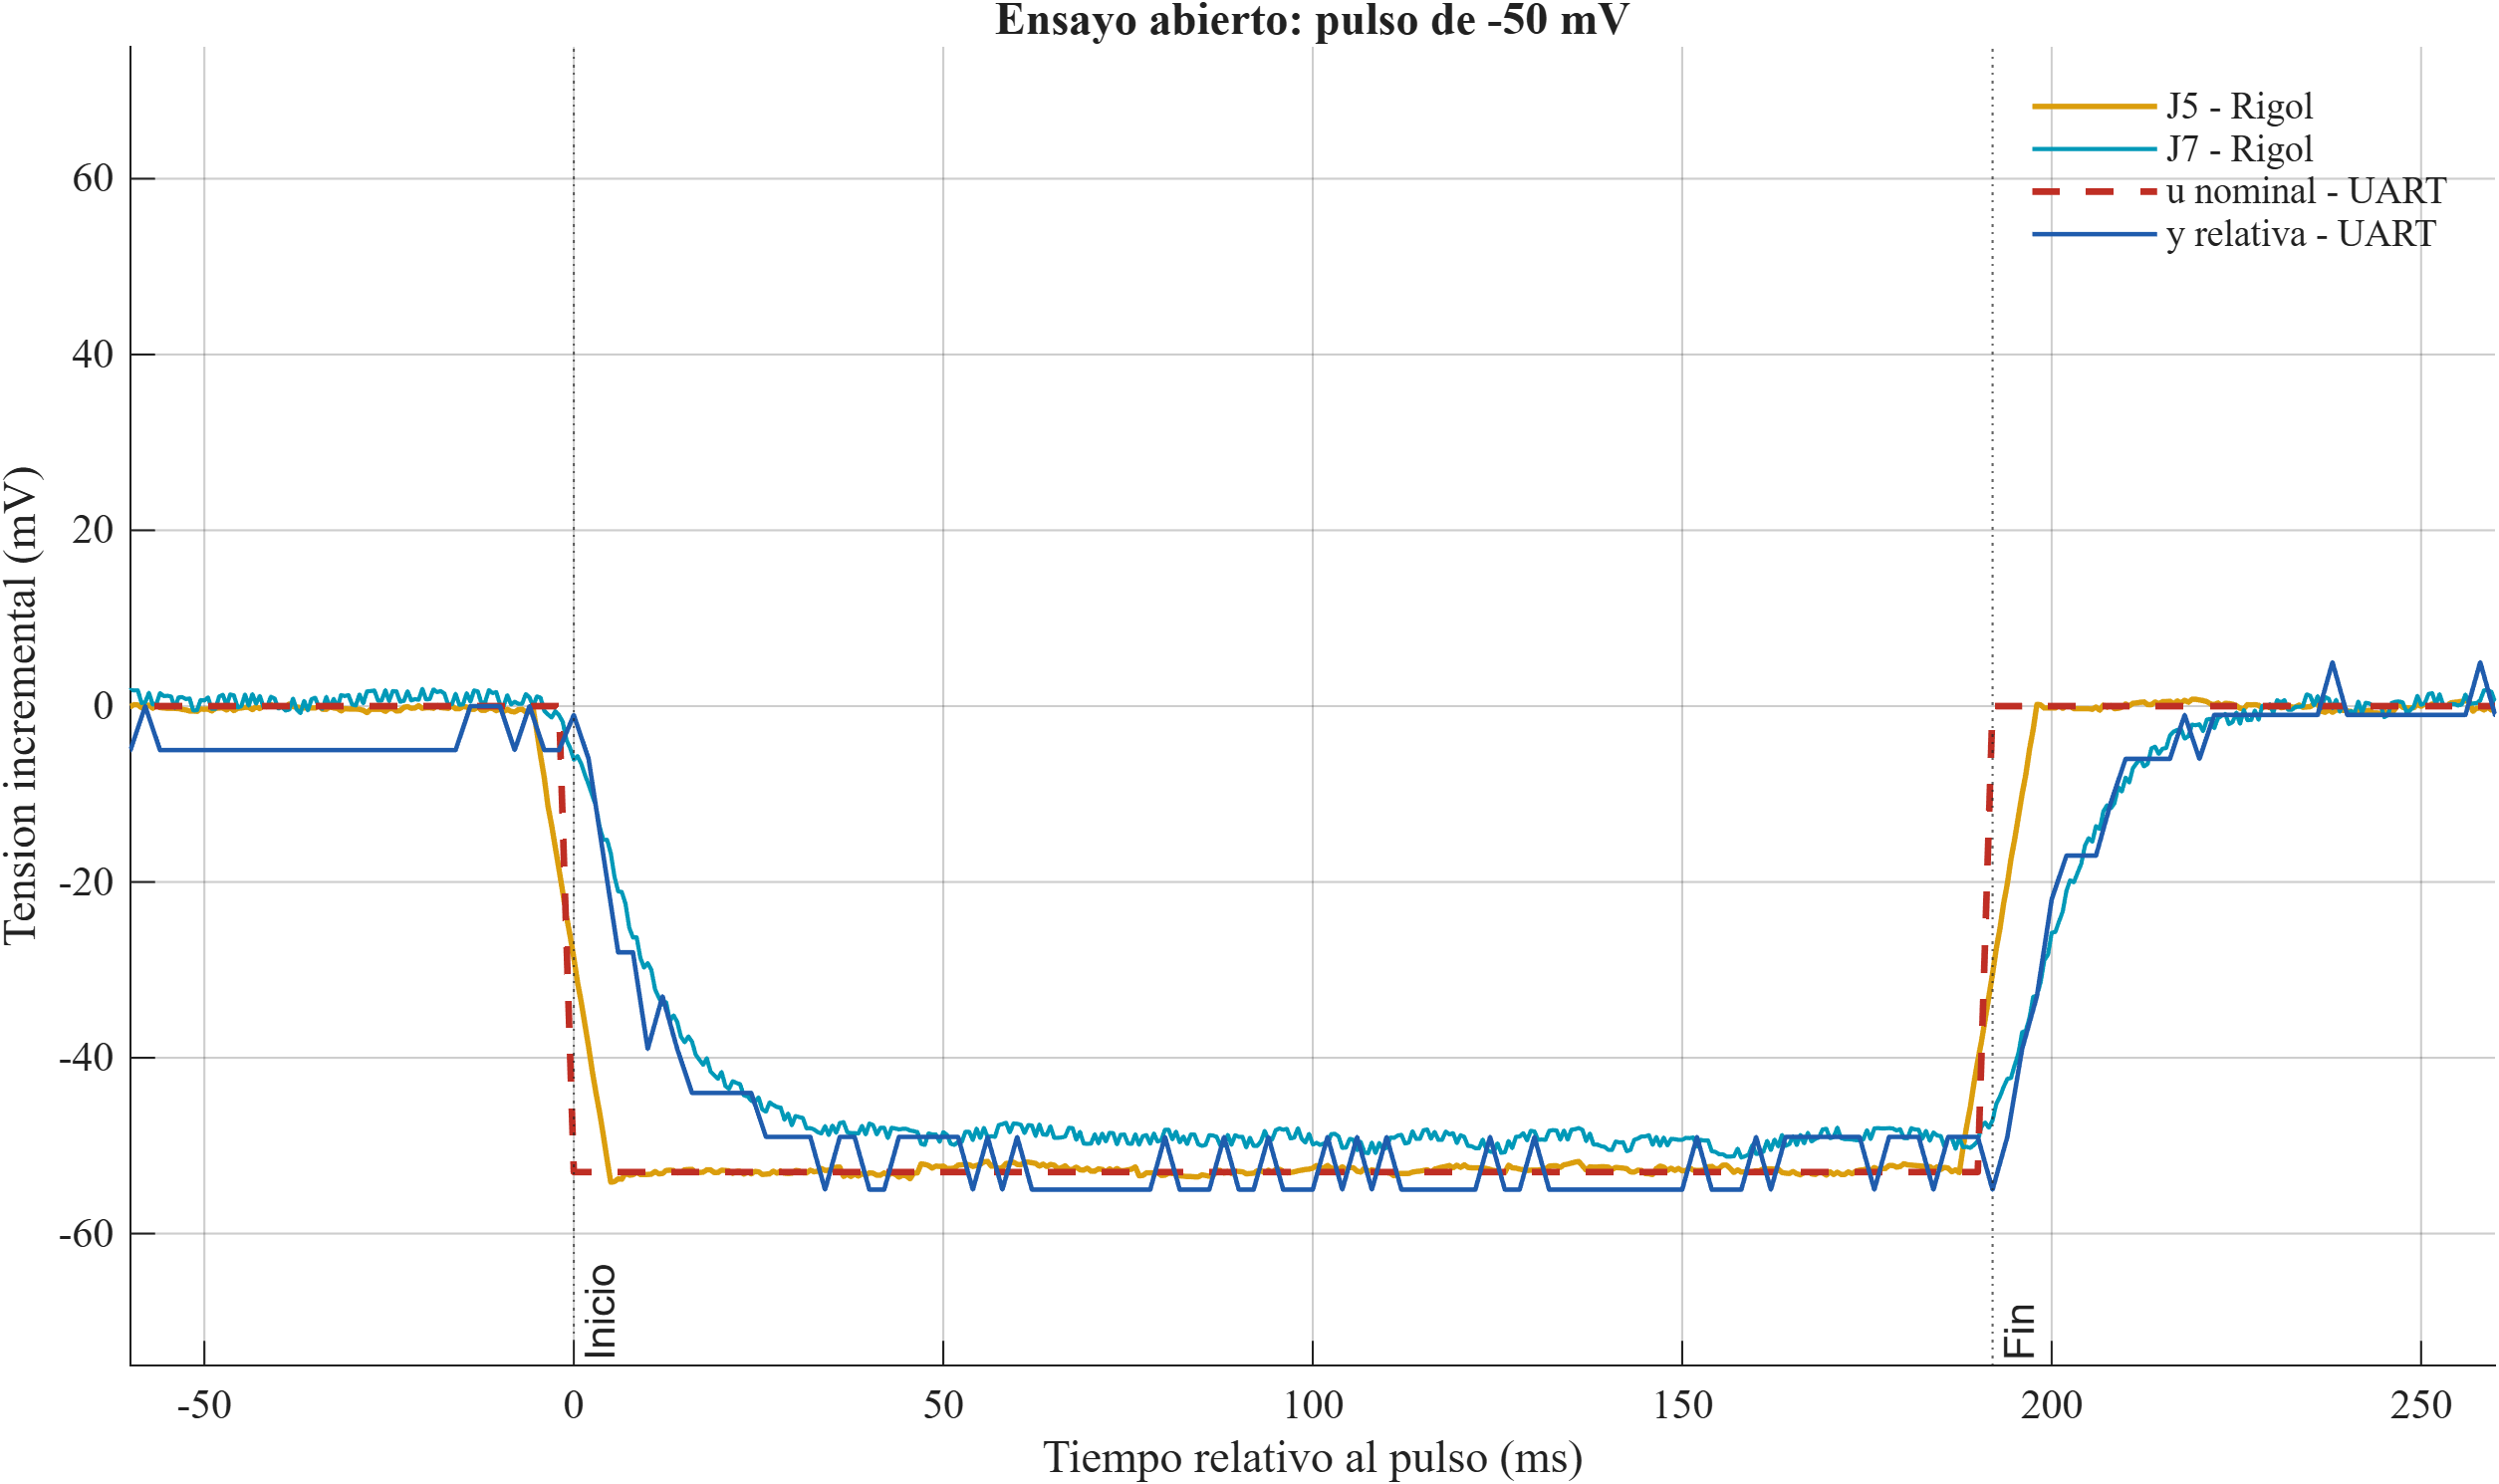
\includegraphics[width=0.94\textwidth]{ensayo_abierto_neg_50mV.png}
\caption{Ensayo abierto negativo: comparación temporal entre J5 y J7 descargados del RIGOL y las variables de entrada y salida registradas por UART.}
\label{fig:abierto-neg}
\end{figure*}

\begin{figure*}[!t]
\centering
\includegraphics[width=0.84\textwidth]{pantalla_rigol_abierto_neg_50mV_original.png}
\caption{Pantalla original del RIGOL durante el ensayo abierto de -50 mV. Se conservan ambos flancos, la meseta completa y el archivo sin posprocesado.}
\label{fig:rigol-abierto-neg}
\end{figure*}

\subsection{Lazo integral lento}
Con el banco ya verificado, se habilitó el modo \texttt{INTEGRAL} con el diseño lento, referencia de \SI{50}{mV}, pretrigger de 32 muestras y retiro de referencia en $k=333$. La adquisición reunió 600 filas UART y 1200 puntos por canal del RIGOL. La salida alcanzó una mediana de \SI{49}{mV} en las últimas 50 muestras de la meseta, con error estacionario de \SI{1}{mV} y error RMS de \SI{3.209}{mV}. El pico de \SI{60}{mV} corresponde a \SI{20}{\percent} de sobrepasamiento y la subida 10--90\% fue de \SI{16}{ms}. Con el criterio estricto de banda del 2\%, el tiempo de establecimiento resultó \SI{590}{ms}: la cuantización y el ruido mantienen excursiones discretas alrededor del valor final hasta casi terminar el pulso, por lo que esta métrica no debe confundirse con lentitud del frente inicial.

La Fig.~\ref{fig:integral-lento} alinea el inicio detectado en el RIGOL con $k=32$ y separa seguimiento y mando. La señal J7 confirma una meseta de \SI{47.2}{mV} y residual de \SI{-0.8}{mV}; las diferencias instantáneas frente a UART son compatibles con filtrado analógico, ruido y cuantización. El mando nominal permaneció entre \SI{-21}{mV} y \SI{77}{mV}, lejos de los límites físicos, y no activó saturación ni anti-windup. El disparo ocurrió después del flanco real debido al ruido del mando; por eso la validación del osciloscopio se recalculó mediante los clústeres de nivel bajo y alto, manteniendo intactos CSV, PNG y metadatos originales.

\begin{figure*}[!t]
\centering
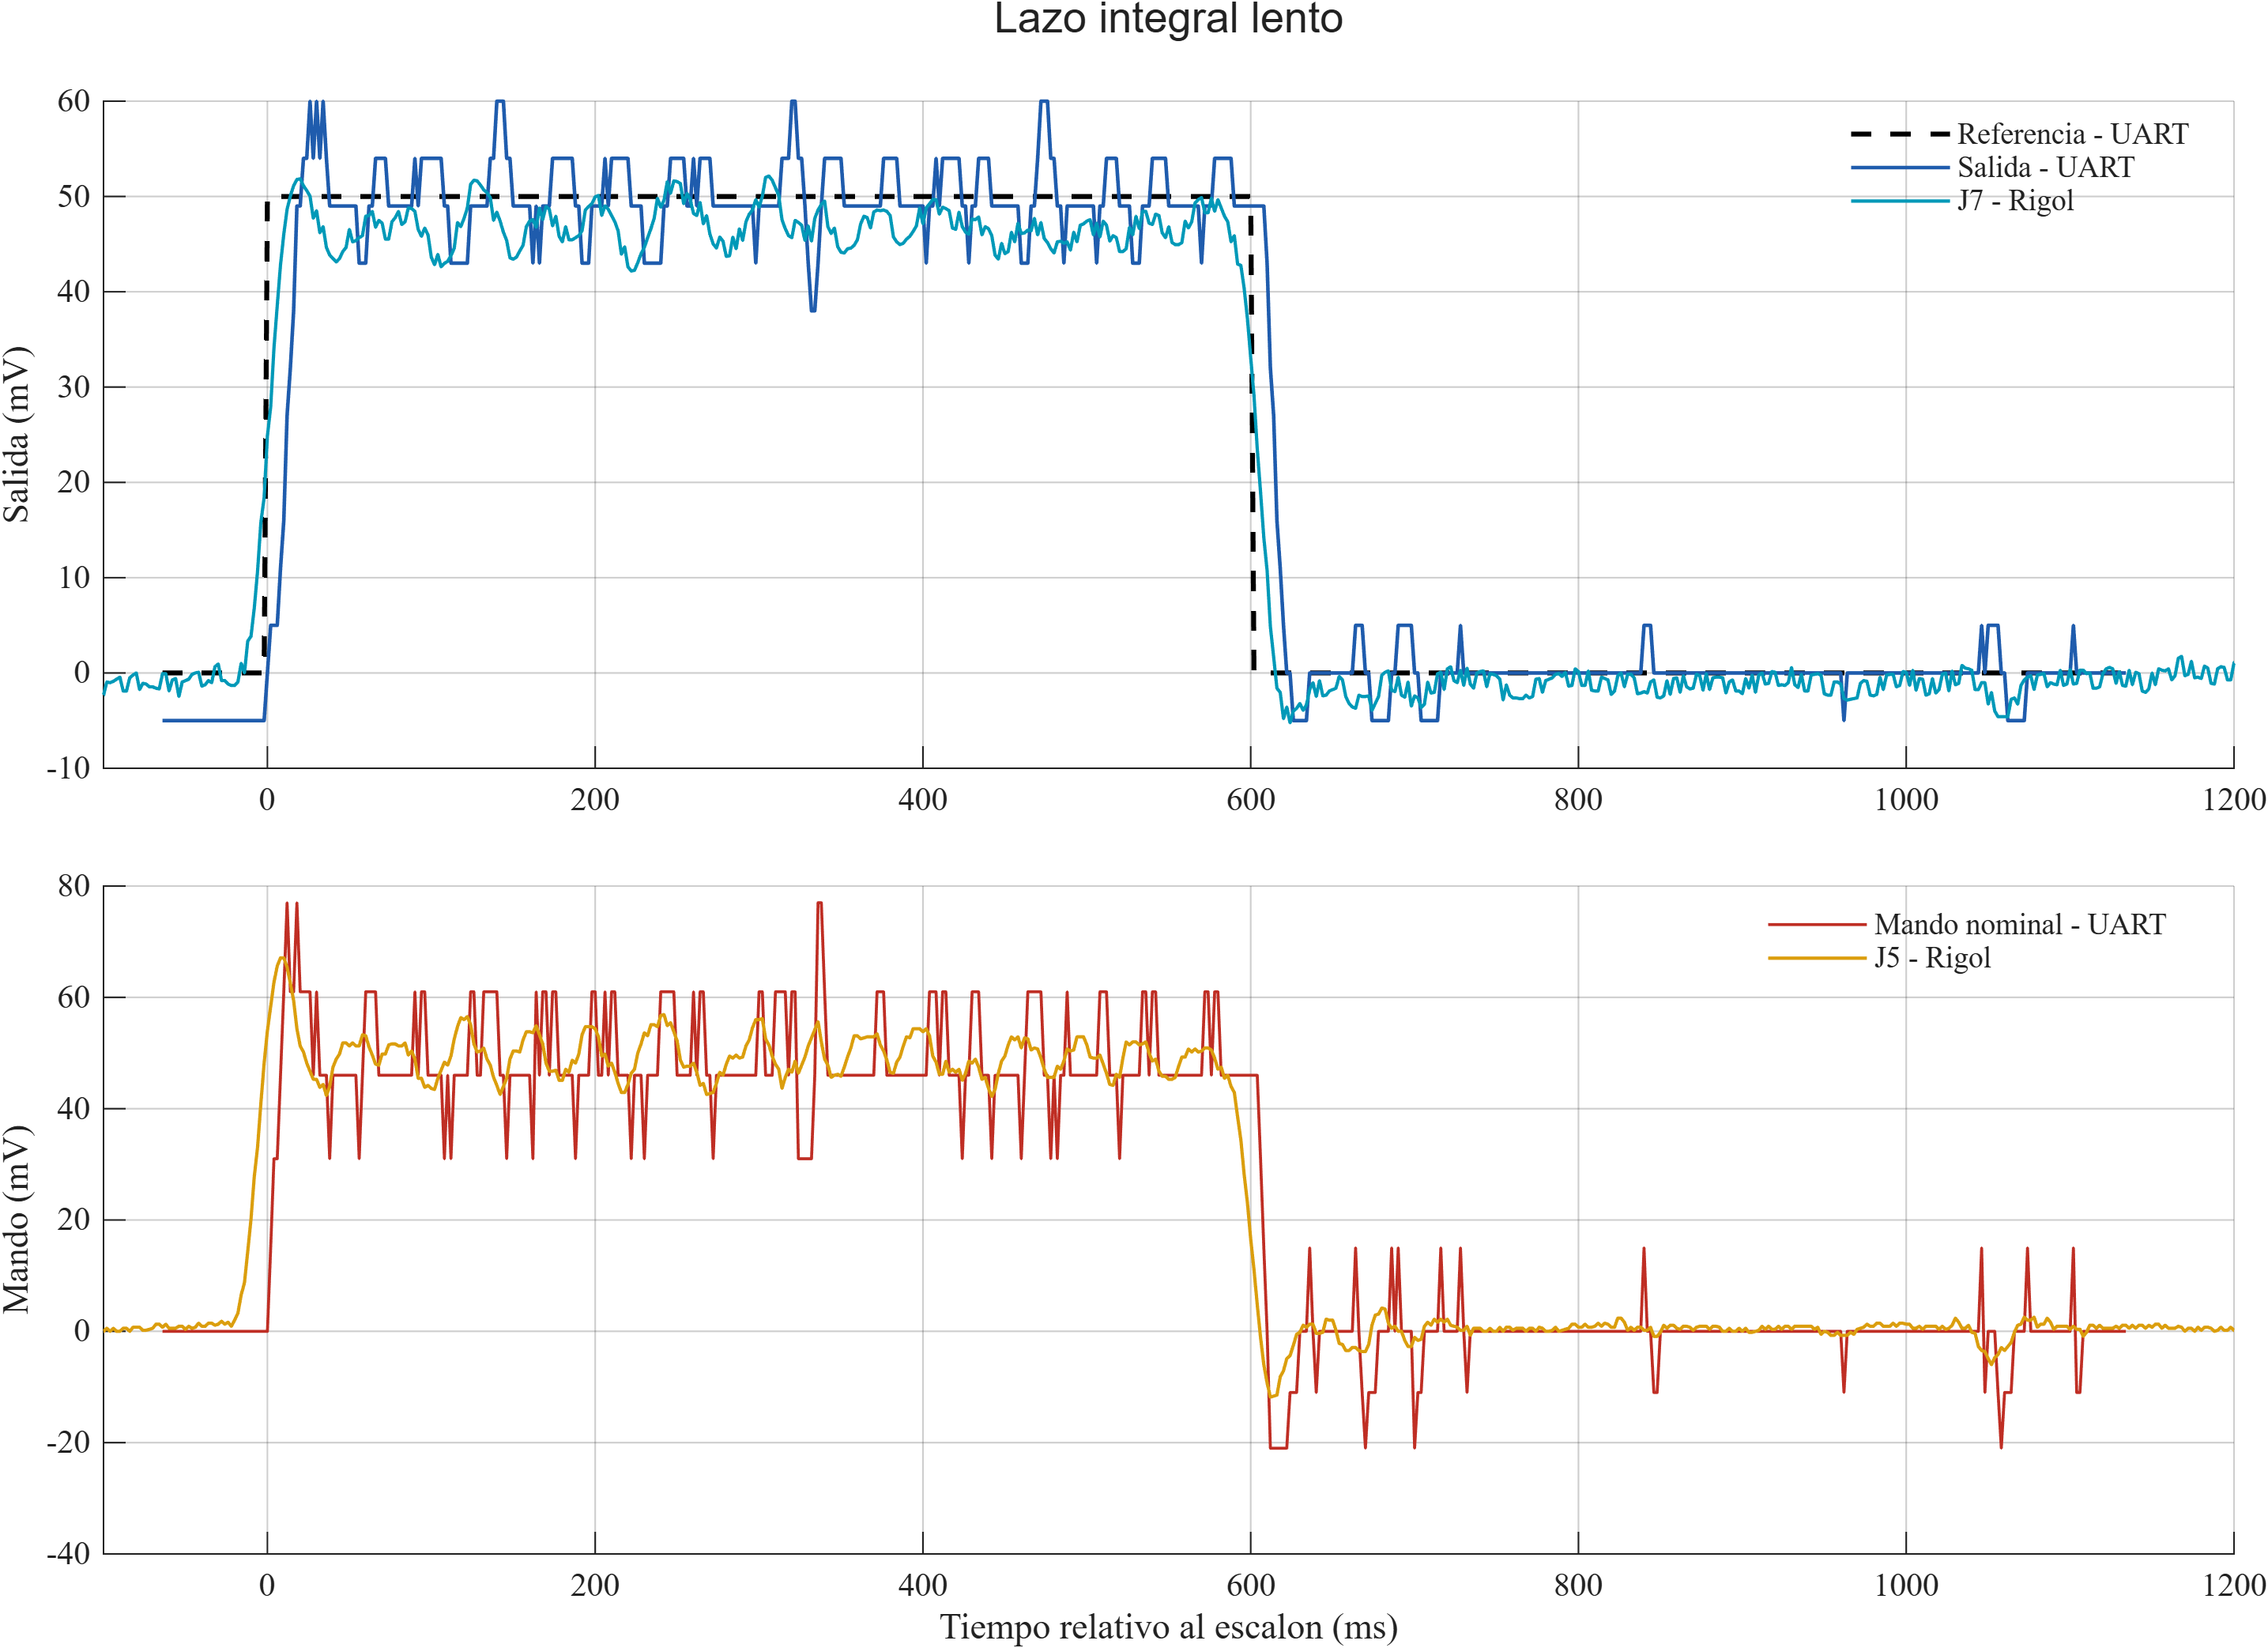
\includegraphics[width=0.88\textwidth]{ensayo_integral_lento.png}\\[0.4em]
\includegraphics[width=0.64\textwidth]{pantalla_rigol_integral_lento_original.png}
\caption{Ensayo integral lento. Arriba: seguimiento y esfuerzo de control registrados por UART y RIGOL. Abajo: pantalla original del osciloscopio, con J5 en CH1 y J7 en CH2.}
\label{fig:integral-lento}
\end{figure*}

\subsection{Lazo integral rápido y comparación}
El mismo protocolo se repitió para el diseño rápido, sin modificar la referencia, el muestreo, el pretrigger ni la duración. Se reunieron nuevamente 600 filas UART, 1200 puntos por canal y la pantalla original. La salida estacionaria fue de \SI{48}{mV}, con error de \SI{2}{mV}, RMS de \SI{2.843}{mV}, pico de \SI{59}{mV}, sobrepasamiento de \SI{18}{\percent} y subida de \SI{12}{ms}. La banda estricta de 2\% no se sostuvo hasta el final del pulso, por lo que $t_s$ se informa como no determinado. El mando nominal quedó entre \SI{-32}{mV} y \SI{77}{mV}, sin saturación, anti-windup ni banderas de falla.

\begin{figure*}[!t]
\centering
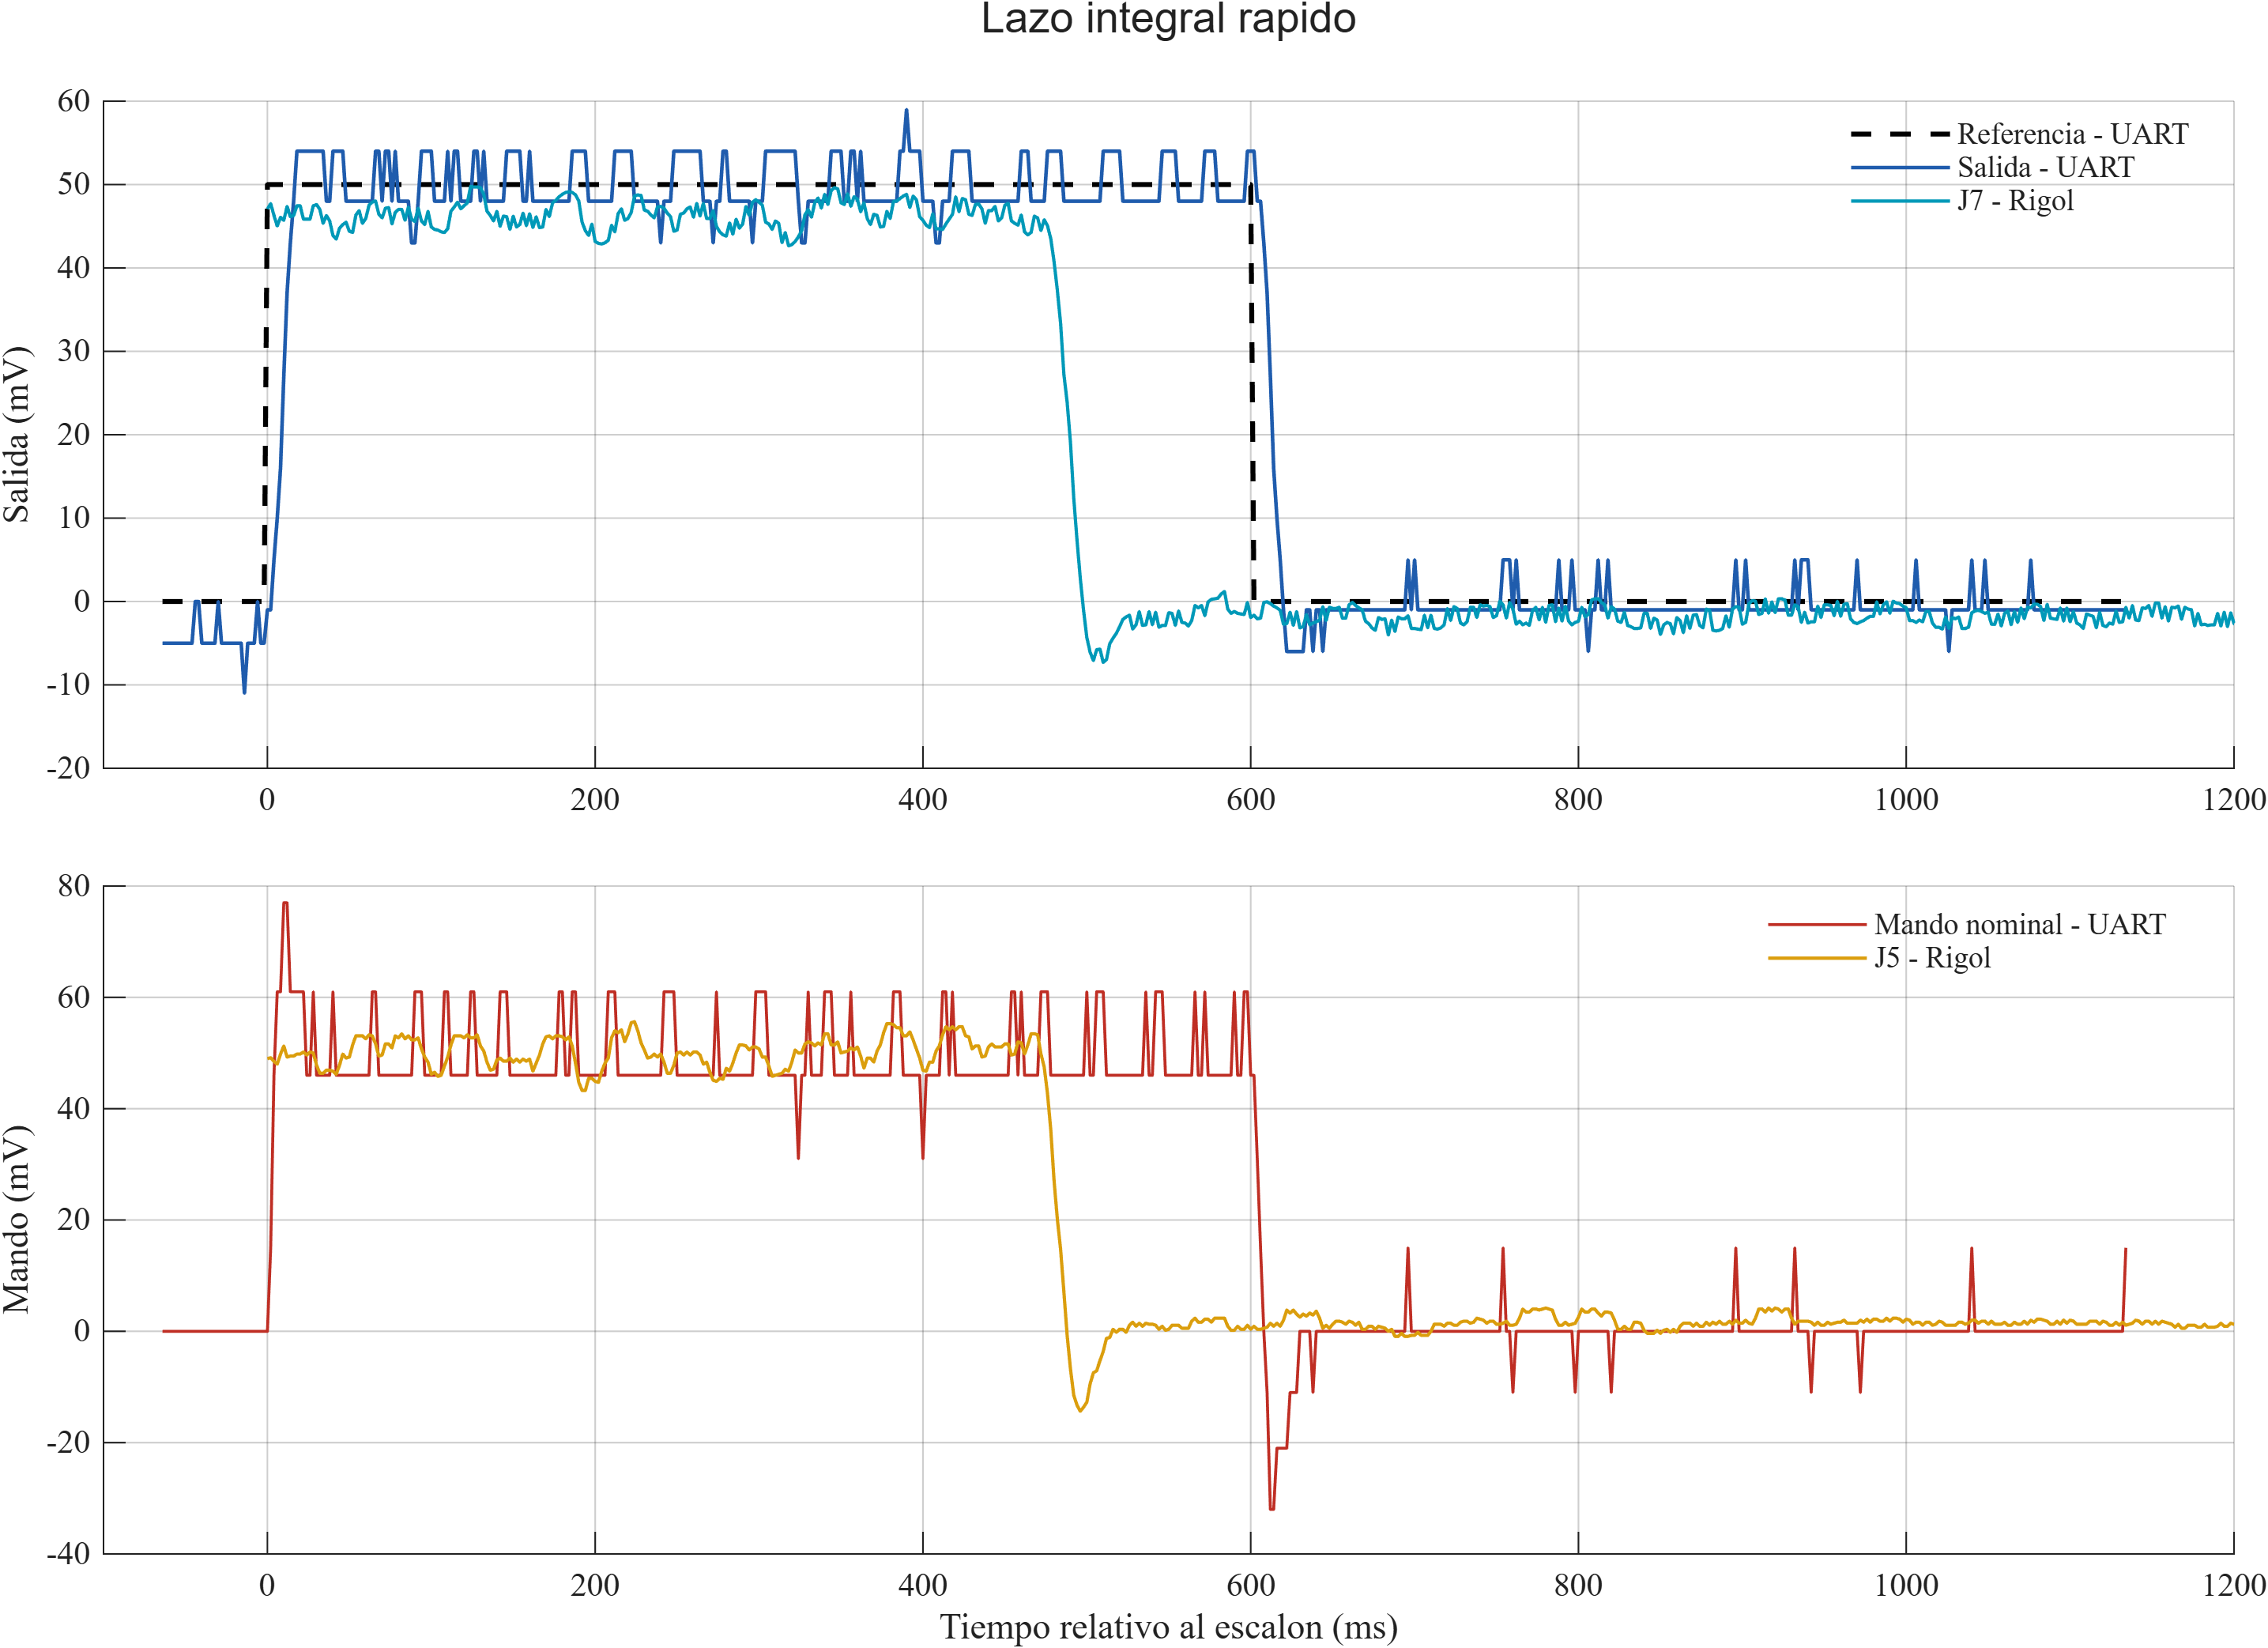
\includegraphics[width=0.88\textwidth]{ensayo_integral_rapido.png}\\[0.4em]
\includegraphics[width=0.64\textwidth]{pantalla_rigol_integral_rapido_original.png}
\caption{Ensayo integral rápido. Arriba: seguimiento y esfuerzo de control registrados por UART y RIGOL. Abajo: pantalla original del osciloscopio, con J5 en CH1 y J7 en CH2.}
\label{fig:integral-rapido}
\end{figure*}

\begin{table}[!t]
\caption{Comparación experimental de los lazos integrales}
\label{tab:comparacion-integral}
\centering
\scriptsize
\begin{tabular}{lrr}
\toprule
Métrica & Lento & Rápido\\
\midrule
Salida estacionaria [mV] & 49 & 48\\
Error estacionario [mV] & 1 & 2\\
Error RMS [mV] & 3.209 & 2.843\\
Subida 10--90\% [ms] & 16 & 12\\
Sobrepasamiento [\%] & 20 & 18\\
Establecimiento 2\% [ms] & 590 & --\\
Mando nominal mín./máx. [mV] & -21 / 77 & -32 / 77\\
Saturación / anti-windup / fallas & 0 / 0 / 0 & 0 / 0 / 0\\
Período mín./med./máx. [$\mu$s] & 1999/2000/2001 & 1999/2000/2001\\
Tiempo máximo ISR [$\mu$s] & 118 & 117\\
$\Delta$J7 / residual RIGOL [mV] & 47.2 / -0.8 & 47.2 / -2.0\\
\bottomrule
\end{tabular}
\end{table}

La Tabla~\ref{tab:sim-exp} coloca los resultados de simulación y de banco bajo las mismas definiciones. Además del criterio estricto del 2\%, se calculó la primera ventana de \SI{20}{ms} en la que al menos el \SI{80}{\percent} de las muestras y su mediana quedan dentro de $\pm\SI{5}{mV}$ de la referencia. Esta medida complementaria permite comparar la llegada práctica a la meseta sin ocultar las oscilaciones pequeñas debidas al ruido y a la cuantización.

\begin{table}[!t]
\caption{Simulación identificada frente al experimento}
\label{tab:sim-exp}
\centering
\scriptsize
\begin{tabular}{lrrrr}
\toprule
Métrica & L--S & L--E & R--S & R--E\\
\midrule
$t_r$ [ms] & 14 & 16 & 10 & 12\\
$M_p$ [\%] & 15.66 & 20.00 & 15.03 & 18.00\\
$e_{ss}$ [mV] & 0.365 & 1.000 & -0.055 & 2.000\\
RMS [mV] & 3.079 & 3.209 & 1.542 & 2.843\\
$u_{\min}$ [mV] & -21.121 & -21.000 & -21.121 & -32.000\\
$u_{\max}$ [mV] & 61.482 & 77.000 & 76.852 & 77.000\\
Ventana $\pm5$ [ms] & 32 & 28 & 24 & 12\\
\bottomrule
\end{tabular}
\begin{flushleft}
\scriptsize L: lento; R: rápido; S: simulación; E: experimento.
\end{flushleft}
\end{table}

La Fig.~\ref{fig:integral-rapido} muestra que el frente inicial rápido requiere \SI{12}{ms} y mantiene una meseta cuantizada comparable a la lenta. El RIGOL midió un incremento de \SI{47.2}{mV} y residual de \SI{-2}{mV}. Su disparo se completó mediante \texttt{TFOR} de respaldo, consignado en los metadatos; los dos niveles y el retorno permanecen visibles en la pantalla original. La comparación confirma una reducción del \SI{25}{\percent} en tiempo de subida y del \SI{11.4}{\percent} en RMS, sin aumentar el máximo positivo ni activar protecciones; a cambio, el mando negativo transitorio pasó de \SI{-21}{mV} a \SI{-32}{mV} y el error estacionario de \SI{1}{mV} a \SI{2}{mV}.

\section{Discusión}
El polo integral rápido reduce el error RMS y acorta el frente, aunque exige un mando negativo transitorio mayor. Con la planta identificada, la simulación presenta $M_p\approx\SI{15}{\percent}$ para ambos controladores y una reducción del tiempo de subida de 14 a \SI{10}{ms}. El ensayo mantuvo la misma tendencia: \SI{16}{ms} frente a \SI{12}{ms}, con \SI{20}{\percent} y \SI{18}{\percent} de sobrepasamiento. Las diferencias entre simulación y banco son mayores en el mando inicial y en el error RMS del diseño rápido; aun así, los signos, el orden relativo de las respuestas y los niveles finales son consistentes. El diseño rápido ofrece una respuesta más breve y un RMS menor, mientras que el lento requiere menos mando negativo y deja un error estacionario un milivoltio menor.

La estabilidad lineal se mantuvo en los cuatro casos ($\rho<1$), aunque esta comprobación por sí sola no representa el ruido ADC, el \emph{jitter}, la deriva de calibración ni las saturaciones físicas. La simulación con cuantización ADC y ruido ubicó el RMS en el mismo orden que los \SI{3.209}{mV} y \SI{2.843}{mV} medidos. Ambos lazos usaron como máximo \SI{77}{mV} y permanecieron lejos de los límites de \SI{-115}{mV}/\SI{107}{mV}. El peor tiempo de ISR fue \SI{118}{\micro s}, equivalente al \SI{5.9}{\percent} de $T_s$, y el período se mantuvo entre \SI{1999}{\micro s} y \SI{2001}{\micro s}. Los sobrepasamientos físicos son algo mayores que el \SI{15}{\percent} previsto, pero no comprometieron la estabilidad ni los límites. Los niveles de \SI{48}{mV}--\SI{49}{mV} por UART y \SI{47.2}{mV} por RIGOL muestran que las dos cadenas de medición describen el mismo comportamiento del sistema.

\section{Conclusiones}
Se completaron el diseño, la simulación y la implementación de dos controladores de seguimiento con acción integral y estimador actual. Los polos calculados coinciden con los valores elegidos dentro de la precisión numérica y el modelo identificado reprodujo mejor los escalones abiertos: su RMSE conjunto fue de \SI{5.756}{mV}, frente a \SI{6.772}{mV} del modelo obtenido a partir de los componentes. MATLAB y Simulink dieron resultados consistentes y permitieron verificar el algoritmo antes de cerrar el lazo en la planta.

El modo \texttt{MONITOR} registró 600 muestras válidas, período mediano de \SI{2}{ms}, variación máxima de \SI{1}{\micro s}, tiempo de ISR de \SI{52}{\micro s}, cero banderas y salida nula. Los ensayos bipolares confirmaron el signo y la escala del DAC en los códigos de trabajo, con diferencias de \SI{3.23}{\percent} y \SI{2.27}{\percent} respecto de los valores usados en la simulación. Esto permitió pasar al lazo cerrado sin modificar las ganancias.

Los controladores lento y rápido siguieron una referencia de \SI{50}{mV} y alcanzaron \SI{49}{mV} y \SI{48}{mV} en régimen. Sus tiempos de subida fueron \SI{16}{ms} y \SI{12}{ms}, mientras que el error RMS fue de \SI{3.209}{mV} y \SI{2.843}{mV}. El diseño rápido redujo el tiempo de subida en \SI{25}{\percent} y el RMS en \SI{11.4}{\percent}; el costo fue aumentar el mando negativo transitorio de \SI{-21}{mV} a \SI{-32}{mV}. En ninguno de los dos casos aparecieron saturaciones, bloqueos de anti-windup ni fallas. El RIGOL midió incrementos de \SI{47.2}{mV} y retornos próximos a cero, lo que confirma el seguimiento estable observado por UART. Para dejar el montaje en una condición segura, el PSoC se programó nuevamente en \texttt{MONITOR} con los enclavamientos de actuación deshabilitados.

\section*{Disponibilidad de artefactos}
Los archivos necesarios para reproducir el trabajo están organizados por etapa:
\begin{itemize}
\item \path{01_Modelado_MATLAB}: diseño, análisis y modelo Simulink;
\item \path{02_Firmware_PSoC_5LP}: workspace y fuentes del PSoC;
\item \path{04_Ensayos}: capturadores, UART, RIGOL y metadatos;
\item \path{05_Resultados}: tablas y figuras procesadas.
\end{itemize}
Cada ensayo conserva 600 filas UART, dos canales de 1200 puntos, los metadatos y la pantalla original del osciloscopio. El archivo \path{README.md} indica el orden de ejecución y los nombres de los scripts.

\begin{thebibliography}{99}
\bibitem{enunciado}
Universidad Católica ``Nuestra Señora de la Asunción'', ``Sistemas de seguimiento--Control integral en el espacio de estados'', enunciado de laboratorio de Automatización, 2026.

\bibitem{ogata}
K. Ogata, \emph{Discrete-Time Control Systems}, 2nd ed. Upper Saddle River, NJ, USA: Prentice Hall, 1995, sec. 6.7.

\bibitem{franklin}
G. F. Franklin, J. D. Powell y M. L. Workman, \emph{Digital Control of Dynamic Systems}, 3rd ed. Menlo Park, CA, USA: Addison-Wesley, 1998, sec. 8.5.

\bibitem{matlab}
MathWorks, ``State-space models, pole placement and Simulink,'' MATLAB and Simulink Documentation, R2026b.

\bibitem{psoc}
Cypress Semiconductor, \emph{PSoC Creator User Guide}, versión 4.4.
\end{thebibliography}

\AddToShipoutPictureFG*{%
  \AtPageLowerLeft{%
    \put(\LenToUnit{\dimexpr\paperwidth-8mm\relax},\LenToUnit{7mm}){%
      \makebox(0,0)[r]{\footnotesize SDG}}}}

\end{document}
